\documentclass[12pt]{article}
\usepackage[utf8]{inputenc}
\usepackage{graphicx}
\usepackage{subcaption}
\usepackage{amsmath}
\usepackage{fancyhdr}
\usepackage{geometry}
\usepackage{dirtytalk}
\usepackage[english]{babel}
\usepackage{csquotes}
\usepackage{hyperref}
\usepackage{listings}
\usepackage{xcolor}
\usepackage{booktabs}
\usepackage{longtable}
\usepackage{array}
\usepackage{tikz}
\usetikzlibrary{shapes.geometric, arrows, positioning, fit}
\usepackage[T1]{fontenc}

\lstset{
    language=C++,
    basicstyle=\ttfamily\small,
    numberstyle=\tiny,
    frame=single,
    breaklines=true,
    commentstyle=\color{green!50!black},
    keywordstyle=\color{blue},
    stringstyle=\color{red},
    showstringspaces=false,
    numbers=left
}

\linespread{1.25}
\setlength{\parindent}{0.8cm}
\setlength{\parskip}{0em}
\renewcommand{\headrulewidth}{0pt}
\geometry{a4paper, portrait, margin=1in}
\setlength{\headheight}{14.49998pt}
\graphicspath{{./}{../}}

% TikZ styles
\tikzstyle{startstop} = [rectangle, rounded corners, minimum width=3cm, minimum height=1cm, text centered, draw=black, fill=red!30]
\tikzstyle{process}   = [rectangle, minimum width=3.2cm, minimum height=1cm, text centered, draw=black, fill=blue!20]
\tikzstyle{decision}  = [diamond, minimum width=3.2cm, minimum height=1cm, text centered, draw=black, fill=green!20]
\tikzstyle{arrow}     = [thick,->,>=stealth]
\tikzstyle{block}     = [rectangle, draw, text width=7em, text centered, rounded corners, minimum height=3em]
\tikzset{every node/.style={align=center}}

% ============================================================================
\begin{document}

% ---------------------------------------------------------------------------
% TITLE PAGE
% ---------------------------------------------------------------------------
\begin{titlepage}
  \begin{center}
    \textsc{\large Ministry of Education of Republic of Moldova}\\[0.5cm]
    \textsc{\large Technical University of Moldova}\\[0.5cm]
    \textsc{\large Faculty of Computers, Informatics and Microelectronics}\\[0.5cm]
    \textsc{\large Software Engineering Department}\\[1.2cm]

    \vspace{20mm}
    \textsc{\Large Embedded Systems}\\[0.5cm]
    \textsc{\large Laboratory Work \#4}\\[0.5cm]

    \newcommand{\HRule}{\rule{\linewidth}{0.5mm}}
    \vspace{8mm}
    \HRule\\[0.4cm]
    {\LARGE \bfseries Button Duration Monitor with FreeRTOS\\[0.2cm]
    \large Preemptive Multitasking with Binary Semaphores and Mutexes\\[0.3cm]}
    \HRule\\[1.5cm]

    \begin{minipage}[t]{0.45\textwidth}
      \begin{flushleft}\large
        \emph{Author:}\\
        Sava \textsc{Luchian}\\
        std. gr. FAF-233
      \end{flushleft}
    \end{minipage}
    ~
    \begin{minipage}[t]{0.45\textwidth}
      \begin{flushright}\large
        \emph{Verified:}\\
        Alexei \textsc{Martiniuc}\\
      \end{flushright}
    \end{minipage}\\[2.5cm]

    \large Chisinau 2026
    \vfill
  \end{center}
\end{titlepage}

\setcounter{page}{2}
\pagestyle{fancy}
\fancyhf{}
\rhead{\thepage}
\lhead{FAF-233 Sava Luchian; Laboratory Work No.\ 4}

% ---------------------------------------------------------------------------
% TECHNICAL TASK
% ---------------------------------------------------------------------------
\section*{Technical Task}

\subsection*{Purpose of the Laboratory}
\hspace{0.8cm} Familiarise students with FreeRTOS preemptive multitasking on embedded microcontrollers by implementing a button duration monitoring application that executes three concurrent tasks, demonstrates inter-task synchronisation using binary semaphores and mutexes, and reports periodic statistics via STDIO using \texttt{printf}.

\subsection*{Objectives}
\begin{enumerate}
    \item Implement a FreeRTOS preemptive application with three dedicated tasks on an Arduino Uno.
    \item Use \texttt{vTaskDelay} and \texttt{vTaskDelayUntil} for task recurrence and initial offset.
    \item Port application logic from bare-metal to FreeRTOS with minimal code changes.
    \item Demonstrate binary semaphore-based event signalling between tasks.
    \item Demonstrate mutex-based protection of shared global variables.
    \item Validate safe resource access and inter-task communication via STDIO output.
\end{enumerate}

\subsection*{Individual Task}
\hspace{0.8cm} Design and implement on an \textbf{Arduino Uno (ATmega328P)} a FreeRTOS preemptive multitasking button monitoring application structured into three tasks:

\begin{itemize}
    \item \textbf{Task 1} -- Detect button press/release with debounce, measure press duration; signal \textbf{Green LED} for short press ($<$\,500\,ms) and \textbf{Red LED} for long press ($\geq$\,500\,ms). Run with \texttt{vTaskDelayUntil} at 20\,ms period.
    \item \textbf{Task 2} -- On each press event (signalled via binary semaphore): increment counters, accumulate duration statistics, and blink the \textbf{Yellow LED} (5$\times$ for short, 10$\times$ for long, 100\,ms blink period using \texttt{vTaskDelay}).
    \item \textbf{Task 3} -- Every 10\,s (via \texttt{vTaskDelayUntil}): acquire mutex, print total presses, short/long counts and average durations to Serial via \texttt{printf}, reset all counters, release mutex.
\end{itemize}

Synchronisation must use a \textbf{binary semaphore} for Task\,1$\rightarrow$Task\,2 event notification and a \textbf{mutex} to protect all accesses to the shared statistics struct.

% ---------------------------------------------------------------------------
% SECTION 1 — DOMAIN ANALYSIS
% ---------------------------------------------------------------------------
\section{Domain Analysis}

\subsection{Technological Context and Application Domain}
\hspace{0.8cm} Preemptive real-time operating systems (RTOS) are the industry-standard solution for embedded applications that must respond to external events within bounded latencies while concurrently managing multiple independent activities. FreeRTOS, the most widely deployed open-source RTOS, is used in millions of products spanning IoT devices, industrial controllers, medical equipment, and automotive body electronics.

This laboratory focuses exclusively on the FreeRTOS model (Part\,2 of the lab specification), investigating:

\begin{itemize}
    \item \textbf{Preemptive scheduling}: The kernel can interrupt a running task at any tick boundary and switch to a higher-priority task. This guarantees latency bounds proportional to task priority, independent of lower-priority task execution time.
    \item \textbf{Event-driven tasks}: A task can block on a synchronisation primitive (semaphore, mutex, queue) releasing the CPU entirely until an event arrives -- the core efficiency advantage over polling.
    \item \textbf{Safe shared memory}: With preemption, two tasks can be context-switched mid-read/write on a multi-byte variable, producing corrupted data. Mutexes eliminate this race condition.
\end{itemize}

\subsection{Hardware Components and Justification}

\begin{table}[h!]
\centering
\begin{tabular}{p{4cm} p{2cm} p{7cm}}
\toprule
\textbf{Component} & \textbf{Qty} & \textbf{Role in the application} \\
\midrule
Arduino Uno (ATmega328P) & 1 & Main MCU; 16\,MHz, 2\,KB SRAM, 32\,KB Flash. FreeRTOS port via feilipu/FreeRTOS. \\
Push-button & 1 & User input; D2 to GND (INPUT\_PULLUP activated). \\
Green LED + 220\,$\Omega$ & 1 & Visual feedback for short press ($<$\,500\,ms). \\
Red LED + 220\,$\Omega$ & 1 & Visual feedback for long press ($\geq$\,500\,ms). \\
Yellow LED + 220\,$\Omega$ & 1 & Statistics blink per press event. \\
Breadboard + jumper wires & -- & Prototyping interconnection. \\
USB cable & 1 & 5\,V power and serial communication (115\,200 baud). \\
\bottomrule
\end{tabular}
\caption{Hardware components used in Lab 4}
\label{tab:hardware}
\end{table}

\subsection{Software Components and Technologies}

\begin{itemize}
    \item \textbf{PlatformIO + VS Code}: Single \texttt{freertos} environment. FreeRTOS heap raised to 950\,bytes to accommodate three tasks, idle task, binary semaphore, and mutex.
    \item \textbf{Arduino Framework (avr-arduino 5.2.0)}: GPIO abstractions, \texttt{Serial}, \texttt{millis()}.
    \item \textbf{feilipu/FreeRTOS 11.1.0-3}: FreeRTOS AVR port; provides \texttt{xTaskCreate}, \texttt{xSemaphoreCreateBinary}, \texttt{xSemaphoreCreateMutex}, \texttt{vTaskDelayUntil}, \texttt{vTaskDelay}.
    \item \textbf{AVR-libc stdio}: \texttt{fdev\_setup\_stream} + \texttt{printf} redirected to Serial UART via a custom \texttt{serial\_putchar} bridge; \texttt{ultoa()} for stack-safe integer formatting.
    \item \textbf{Wokwi Simulator}: Circuit + firmware simulation in VS Code for functional testing.
\end{itemize}

\subsection{Analysis of Existing Solutions}
\hspace{0.8cm} The key advantage of FreeRTOS over a bare-metal scheduler for this application is the event-driven blocking model:

\begin{itemize}
    \item \textbf{Bare-metal polling (Part 1)}: Task\,2 must poll \texttt{newPressAvailable} every 20\,ms even when no press has occurred -- wasting CPU cycles. In FreeRTOS, Task\,2 blocks on \texttt{xButtonSemaphore} consuming zero CPU while idle.
    \item \textbf{FreeRTOS queues}: Could replace the semaphore + shared struct with a typed message queue, enabling loss-less buffering of multiple rapid presses. For this application a semaphore + mutex is sufficient and more resource-efficient on the 2\,KB SRAM ATmega328P.
    \item \textbf{Cooperative FreeRTOS}: Tasks can voluntarily yield but the scheduler does not preempt -- removing the need for mutexes. Not chosen because preemption provides better latency and is the standard FreeRTOS configuration.
\end{itemize}

\subsection{Real-World Applications}
\hspace{0.8cm} The design patterns demonstrated in this laboratory appear directly in commercial embedded products:

\begin{itemize}
    \item \textbf{IoT sensor nodes (ESP32/STM32)}: AWS FreeRTOS uses exactly the binary-semaphore event model for MQTT publish/subscribe task communication.
    \item \textbf{Home automation hubs}: A button scanning task (like Task\,1) signals a UI management task (like Task\,2) via semaphore on each input event.
    \item \textbf{Motor controllers}: A measurement task publishes feedback data under a mutex; a control task reads it without halting measurement -- the same mutex pattern as \texttt{xStatsMutex}.
    \item \textbf{Medical device firmware}: \texttt{vTaskDelayUntil} is the standard FreeRTOS pattern for fixed-rate sampling loops because it compensates for execution jitter, giving drift-free periods -- critical for waveform-based diagnostics.
    \item \textbf{Vehicle body control modules}: Event semaphores decouple interrupt service routines (physical button debounce handled in hardware on production MCUs) from application task processing, matching the Task\,1/Task\,2 split here.
    \item \textbf{Industrial HMI panels}: A statistics/logging task (like Task\,3) wakes periodically to flush buffered data to persistent storage or a remote server, using a mutex to snapshot the shared counter state cleanly.
\end{itemize}

% ---------------------------------------------------------------------------
% SECTION 2 — CONCEPTUALISATION AND DESIGN
% ---------------------------------------------------------------------------
\section{Conceptualisation and Design}

\subsection{Technical Requirements}

\begin{longtable}{p{1.5cm} p{2.5cm} p{7.5cm} p{1.5cm}}
\toprule
\textbf{ID} & \textbf{Category} & \textbf{Requirement} & \textbf{Type} \\
\midrule
\endfirsthead
R-F-01 & Button & System shall detect button press and release with software debounce (stable $\geq$\,20\,ms). & Func. \\
R-F-02 & Button & System shall measure press duration in milliseconds from first stable press to first stable release. & Func. \\
R-F-03 & LED & Green LED shall illuminate for 800\,ms after a short press ($<$\,500\,ms). & Func. \\
R-F-04 & LED & Red LED shall illuminate for 800\,ms after a long press ($\geq$\,500\,ms). & Func. \\
R-F-05 & Statistics & System shall count and accumulate total, short, and long presses and duration sums. & Func. \\
R-F-06 & LED & Yellow LED shall blink 5 times at 100\,ms ON/OFF after each short press. & Func. \\
R-F-07 & LED & Yellow LED shall blink 10 times at 100\,ms ON/OFF after each long press. & Func. \\
R-F-08 & Report & System shall print statistics via \texttt{printf} (STDIO) every 10\,s: total, short, long counts and average durations. & Func. \\
R-F-09 & Report & System shall reset all counters to zero immediately after each report. & Func. \\
R-F-10 & Sync & Task\,1 shall signal Task\,2 using a binary semaphore after each detected press. & Func. \\
R-F-11 & Sync & All accesses to \texttt{gShared} statistics fields shall be protected by \texttt{xStatsMutex}. & Func. \\
R-F-12 & Scheduling & Task\,1 shall use \texttt{vTaskDelayUntil} for 20\,ms periodic scheduling. & Func. \\
R-F-13 & Scheduling & Task\,3 shall use \texttt{vTaskDelayUntil} for drift-free 10\,s periodic reporting. & Func. \\
R-NF-01 & Latency & Maximum latency from button edge to LED response shall be $<$\,100\,ms. & Non-func. \\
R-NF-02 & Memory & Firmware shall fit within 32\,KB Flash and 2\,KB SRAM. & Non-func. \\
R-NF-03 & Modularity & Application shall be structured in dedicated modules (config, peripherals, shared, tasks). & Non-func. \\
R-NF-04 & STDIO & All text output shall use \texttt{printf} via a \texttt{stdout} $\rightarrow$ Serial bridge. & Non-func. \\
\bottomrule
\caption{Technical requirements for Lab 4}
\label{tab:requirements}
\end{longtable}

\subsection{Architectural Design}

\subsubsection{System Structural Architecture}

The application follows a four-layer hardware--software boundary:

\begin{figure}[h!]
\centering
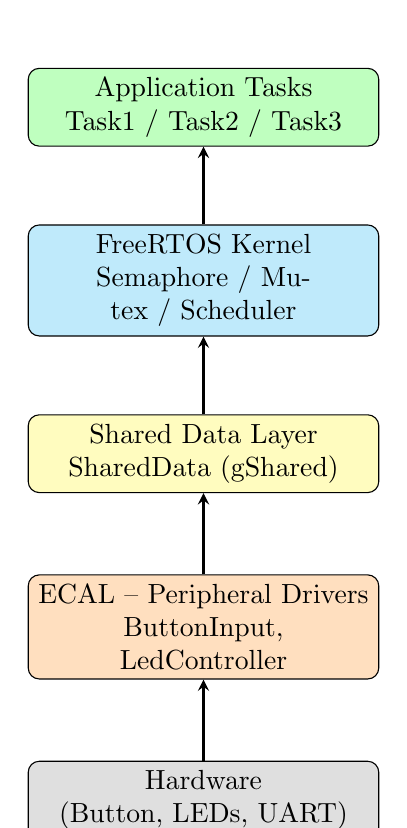
\begin{tikzpicture}
    \node (hw)     at (0, 0)   [block, fill=gray!25,   text width=12em, minimum height=2em]
          {Hardware\\(Button, LEDs, UART)};
    \node (ecal)   at (0, 2.2) [block, fill=orange!25, text width=12em, minimum height=2em]
          {ECAL -- Peripheral Drivers\\ButtonInput, LedController};
    \node (shared) at (0, 4.4) [block, fill=yellow!25, text width=12em, minimum height=2em]
          {Shared Data Layer\\SharedData (gShared)};
    \node (rtos)   at (0, 6.6) [block, fill=cyan!25,   text width=12em, minimum height=2em]
          {FreeRTOS Kernel\\Semaphore / Mutex / Scheduler};
    \node (tasks)  at (0, 8.8) [block, fill=green!25,  text width=12em, minimum height=2em]
          {Application Tasks\\Task1 / Task2 / Task3};

    \draw [arrow] (hw)     -- (ecal);
    \draw [arrow] (ecal)   -- (shared);
    \draw [arrow] (shared) -- (rtos);
    \draw [arrow] (rtos)   -- (tasks);
\end{tikzpicture}
\caption{Layered software architecture -- FreeRTOS}
\label{fig:layers}
\end{figure}

\subsubsection{HW/SW Interface and Component Interaction}

\begin{figure}[h!]
\centering
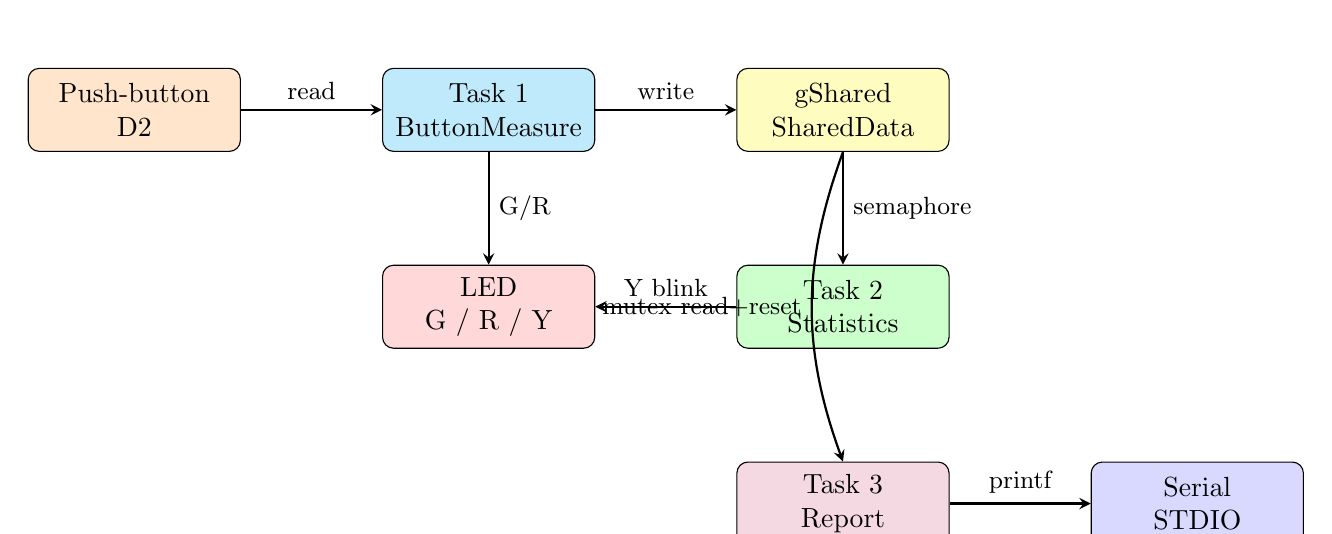
\begin{tikzpicture}
    \node (btn)     at (0,0)     [block, fill=orange!20] {Push-button\\D2};
    \node (task1)   at (4.5,0)   [block, fill=cyan!25]   {Task 1\\ButtonMeasure};
    \node (gshared) at (9.0,0)   [block, fill=yellow!25] {gShared\\SharedData};
    \node (leds)    at (4.5,-2.5)[block, fill=red!15]    {LED\\G / R / Y};
    \node (task2)   at (9.0,-2.5)[block, fill=green!20]  {Task 2\\Statistics};
    \node (task3)   at (9.0,-5.0)[block, fill=purple!15] {Task 3\\Report};
    \node (serial)  at (13.5,-5.0)[block, fill=blue!15]  {Serial\\STDIO};

    \draw [arrow] (btn)     -- node[above]{\small read}       (task1);
    \draw [arrow] (task1)   -- node[above]{\small write}      (gshared);
    \draw [arrow] (task1)   -- node[right]{\small G/R}        (leds);
    \draw [arrow] (gshared) -- node[right]{\small semaphore}  (task2);
    \draw [arrow] (task2)   -- node[above]{\small Y blink}    (leds);
    \draw [arrow] (gshared.south) to[bend right=20] node[left]{\small mutex read+reset} (task3.north);
    \draw [arrow] (task3)   -- node[above]{\small printf}     (serial);
\end{tikzpicture}
\caption{Component interaction diagram}
\label{fig:interaction}
\end{figure}

\subsubsection{FreeRTOS Task and Synchronisation Design}

Each task is created with \texttt{xTaskCreate()} before \texttt{vTaskStartScheduler()} is called. Two synchronisation primitives are created in \texttt{setup()}: a binary semaphore for inter-task event signalling and a mutex for shared data protection.

\begin{table}[h!]
\centering
\begin{tabular}{lllll}
\toprule
\textbf{Task} & \textbf{Entry Point} & \textbf{Priority} & \textbf{Stack} & \textbf{Scheduling} \\
\midrule
Task 1 & \texttt{task\_button\_rtos} & 2 & 60 words & \texttt{vTaskDelayUntil}, 20\,ms \\
Task 2 & \texttt{task\_stats\_rtos}  & 2 & 60 words & Blocks on \texttt{xButtonSemaphore} \\
Task 3 & \texttt{task\_report\_rtos} & 1 & 200 words & \texttt{vTaskDelayUntil}, 10\,s \\
\bottomrule
\end{tabular}
\caption{FreeRTOS task configuration}
\label{tab:tasks}
\end{table}

Tasks\,1 and 2 share the same priority (2) to prevent Task\,1 from starving Task\,2 when the CPU is handed off via the binary semaphore. Task\,3 runs at lower priority (1) so statistics reporting never delays button detection.

\begin{table}[h!]
\centering
\begin{tabular}{llll}
\toprule
\textbf{Primitive} & \textbf{Name} & \textbf{Give (signal)} & \textbf{Take (wait)} \\
\midrule
Binary semaphore & \texttt{xButtonSemaphore} & Task 1 -- after every press & Task 2 -- event-driven \\
Mutex & \texttt{xStatsMutex} & Any after access & Task 1, 2, 3 before \texttt{gShared} access \\
\bottomrule
\end{tabular}
\caption{FreeRTOS synchronisation primitives}
\label{tab:sync}
\end{table}

Task\,2 blocks indefinitely on \texttt{xButtonSemaphore} with \texttt{portMAX\_DELAY} -- consuming zero CPU while no press has been detected. This is the key event-driven efficiency of FreeRTOS versus the bare-metal polling model.

\subsubsection{STDIO Bridge Design}

On AVR the standard C \texttt{printf} function writes to \texttt{stdout}. The Arduino framework does not redirect \texttt{stdout} by default. A custom \texttt{serial\_putchar} function registered via \texttt{fdev\_setup\_stream} translates each character write to \texttt{Serial.write()}, with automatic \texttt{\textbackslash{}n} $\rightarrow$ \texttt{\textbackslash{}r\textbackslash{}n} conversion for correct terminal line endings. This bridge is established once in \texttt{setup()} before the FreeRTOS scheduler starts, and all tasks inherit it automatically.

Because the AVR long-integer formatter in \texttt{vfprintf} requires $\approx$\,300\,bytes of call-stack at runtime, \texttt{uint32\_t} values are converted with \texttt{ultoa()} and printed as \texttt{\%s} to prevent stack overflow in the report task stack.

\subsection{Behavioural Modelling}

\subsubsection{ButtonInput Debounce FSM}

\begin{figure}[h!]
\centering
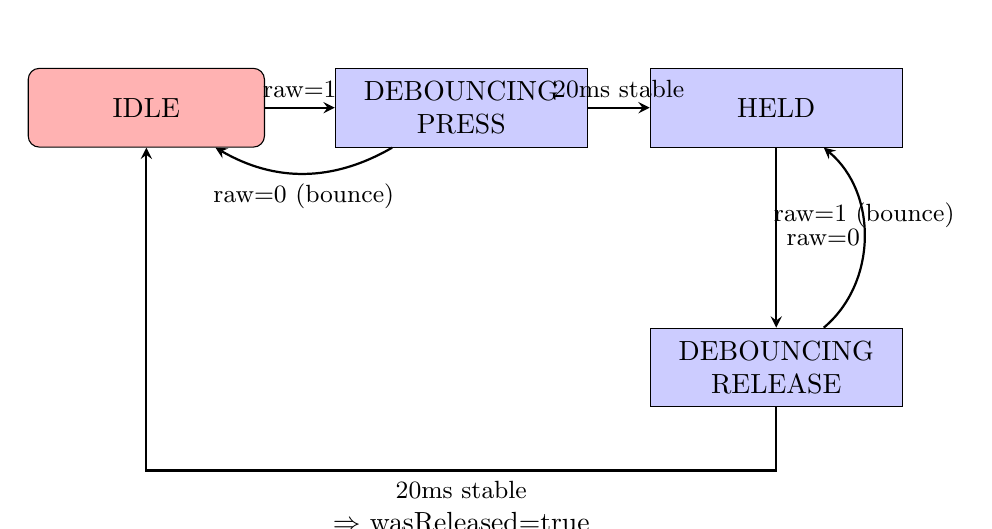
\begin{tikzpicture}[node distance=3cm, auto]
    \node[startstop] (idle)  {IDLE};
    \node[process]   (dp)    [right of=idle, xshift=1cm]  {DEBOUNCING\\PRESS};
    \node[process]   (held)  [right of=dp,   xshift=1cm]  {HELD};
    \node[process]   (dr)    [below of=held, yshift=-0.3cm] {DEBOUNCING\\RELEASE};

    \draw [arrow] (idle) -- node{\small raw=1} (dp);
    \draw [arrow] (dp)   to[bend left] node[below]{\small raw=0 (bounce)} (idle);
    \draw [arrow] (dp)   -- node{\small 20ms stable} (held);
    \draw [arrow] (held) -- node[right]{\small raw=0} (dr);
    \draw [arrow] (dr)   to[bend right=50] node[above]{\small raw=1 (bounce)} (held);
    \draw [arrow] (dr.south) -- ++(0,-0.8) -| node[pos=0.25,below]{\small 20ms stable\\$\Rightarrow$ wasReleased=true} (idle.south);
\end{tikzpicture}
\caption{ButtonInput debounce finite-state machine}
\label{fig:button-fsm}
\end{figure}

\subsubsection{Task 1 Flowchart (FreeRTOS)}

\begin{figure}[h!]
\centering
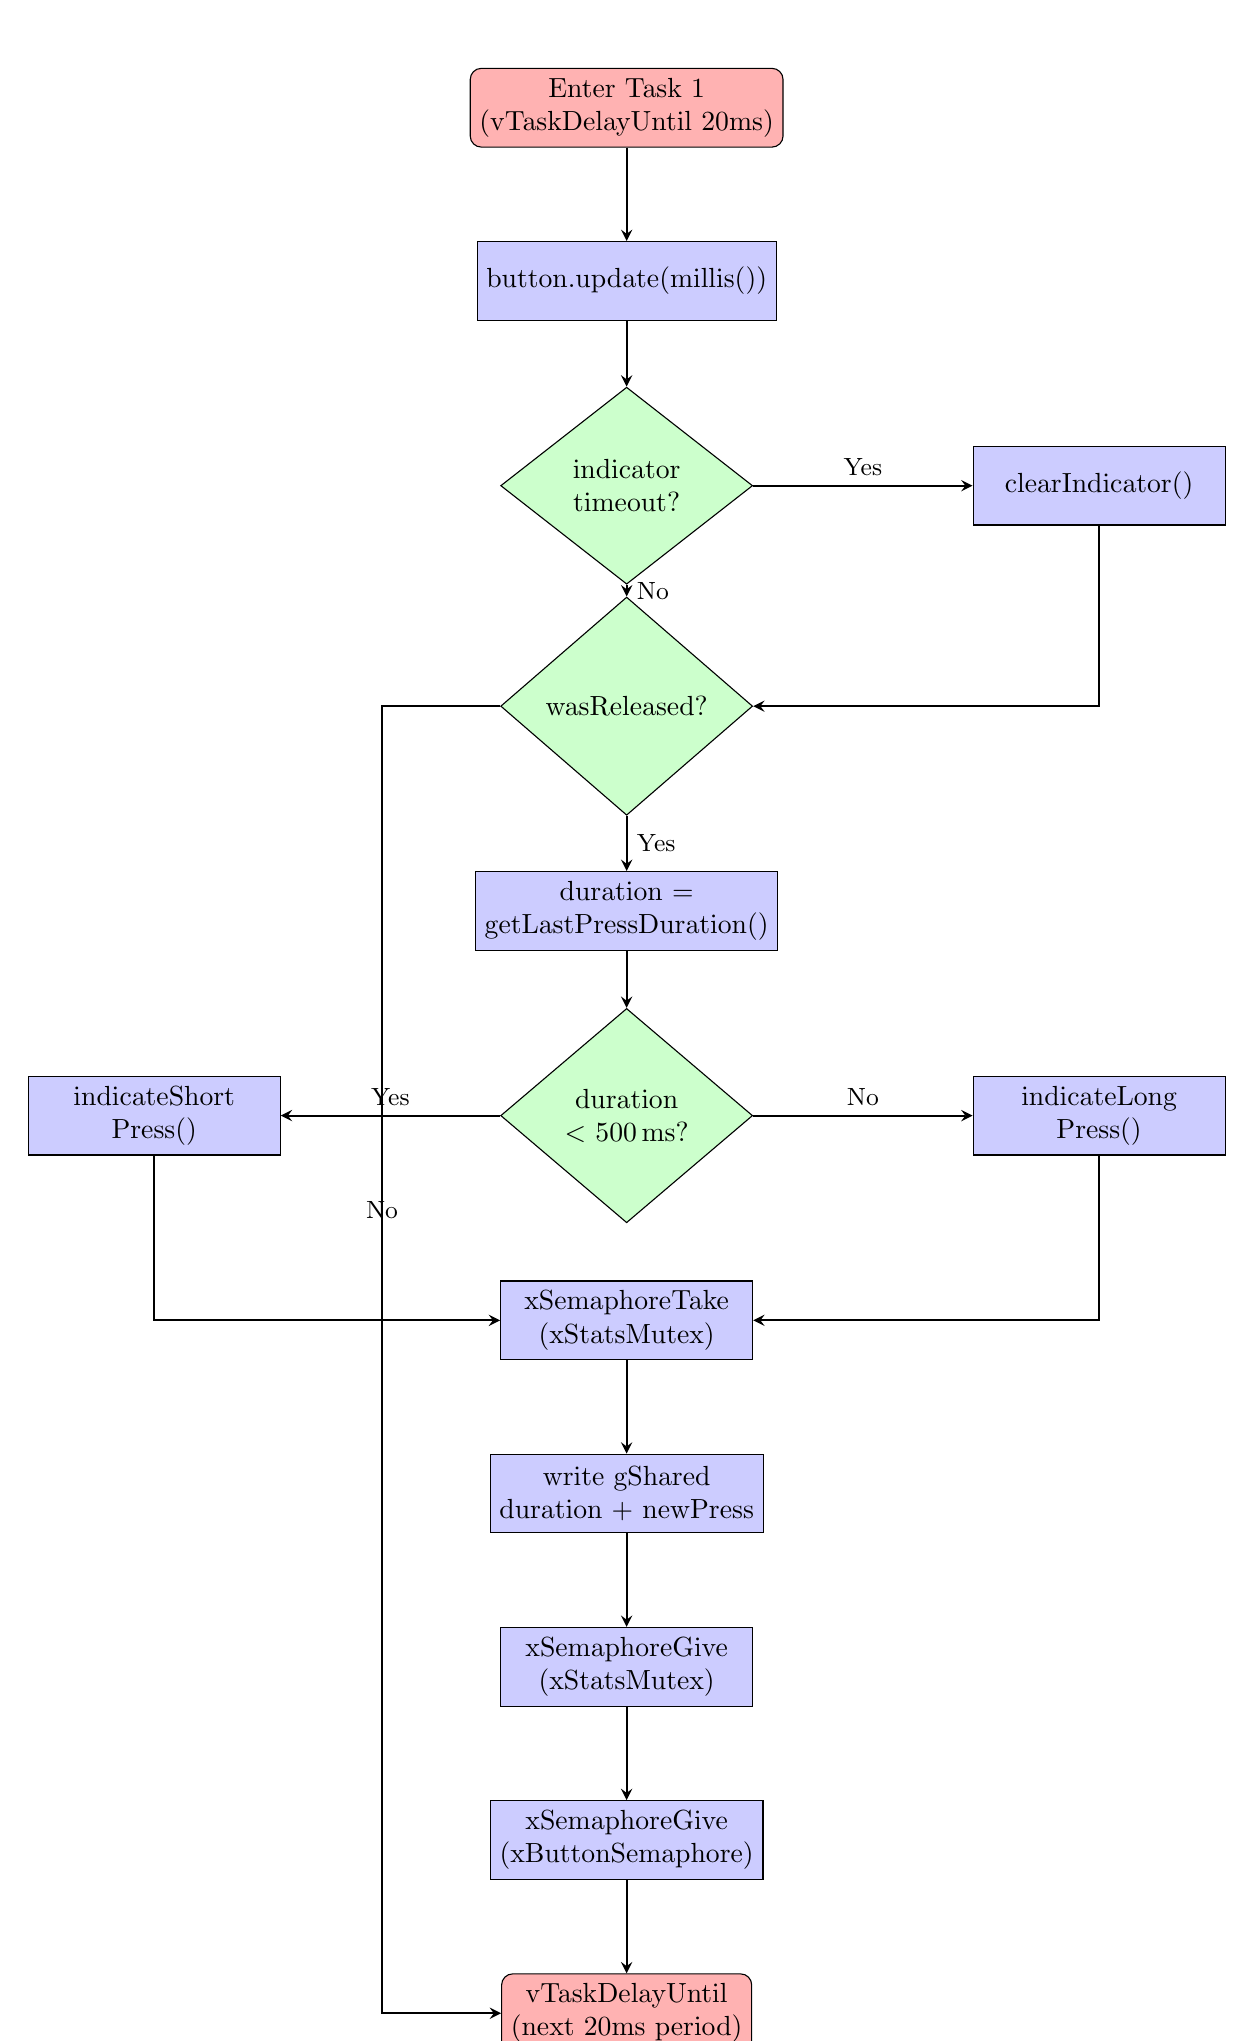
\begin{tikzpicture}
    \node (s)   at ( 0,    0)    [startstop] {Enter Task 1\\(vTaskDelayUntil 20ms)};
    \node (upd) at ( 0,   -2.2)  [process]   {button.update(millis())};
    \node (led) at ( 0,   -4.8)  [decision]  {indicator\\timeout?};
    \node (clr) at ( 6.0, -4.8)  [process]   {clearIndicator()};
    \node (rel) at ( 0,   -7.6)  [decision]  {wasReleased?};
    \node (dur) at ( 0,  -10.2)  [process]   {duration =\\getLastPressDuration()};
    \node (sht) at ( 0,  -12.8)  [decision]  {duration\\$<$ 500\,ms?};
    \node (grn) at (-6.0,-12.8)  [process]   {indicateShort\\Press()};
    \node (red) at ( 6.0,-12.8)  [process]   {indicateLong\\Press()};
    \node (mtx) at ( 0,  -15.4)  [process]   {xSemaphoreTake\\(xStatsMutex)};
    \node (pub) at ( 0,  -17.6)  [process]   {write gShared\\duration + newPress};
    \node (rel2)at ( 0,  -19.8)  [process]   {xSemaphoreGive\\(xStatsMutex)};
    \node (sig) at ( 0,  -22.0)  [process]   {xSemaphoreGive\\(xButtonSemaphore)};
    \node (ret) at ( 0,  -24.2)  [startstop] {vTaskDelayUntil\\(next 20ms period)};

    \draw [arrow] (s)   -- (upd);
    \draw [arrow] (upd) -- (led);
    \draw [arrow] (led) -- node[above]{\small Yes} (clr);
    \draw [arrow] (clr.south) |- (rel.east);
    \draw [arrow] (led) -- node[right]{\small No}  (rel);
    \draw [arrow] (rel) -- node[right]{\small Yes} (dur);
    \draw [arrow] (rel.west) -- ++(-1.5,0) |- node[pos=0.2,above]{\small No} (ret.west);
    \draw [arrow] (dur) -- (sht);
    \draw [arrow] (sht) -- node[above]{\small Yes} (grn);
    \draw [arrow] (sht) -- node[above]{\small No}  (red);
    \draw [arrow] (grn.south) |- (mtx.west);
    \draw [arrow] (red.south) |- (mtx.east);
    \draw [arrow] (mtx) -- (pub);
    \draw [arrow] (pub) -- (rel2);
    \draw [arrow] (rel2)-- (sig);
    \draw [arrow] (sig) -- (ret);
\end{tikzpicture}
\caption{Task 1 flowchart -- button detection, LED signalling, mutex write, semaphore give}
\label{fig:task1flow}
\end{figure}

\subsubsection{Task 2 Flowchart (FreeRTOS)}

\begin{figure}[h!]
\centering
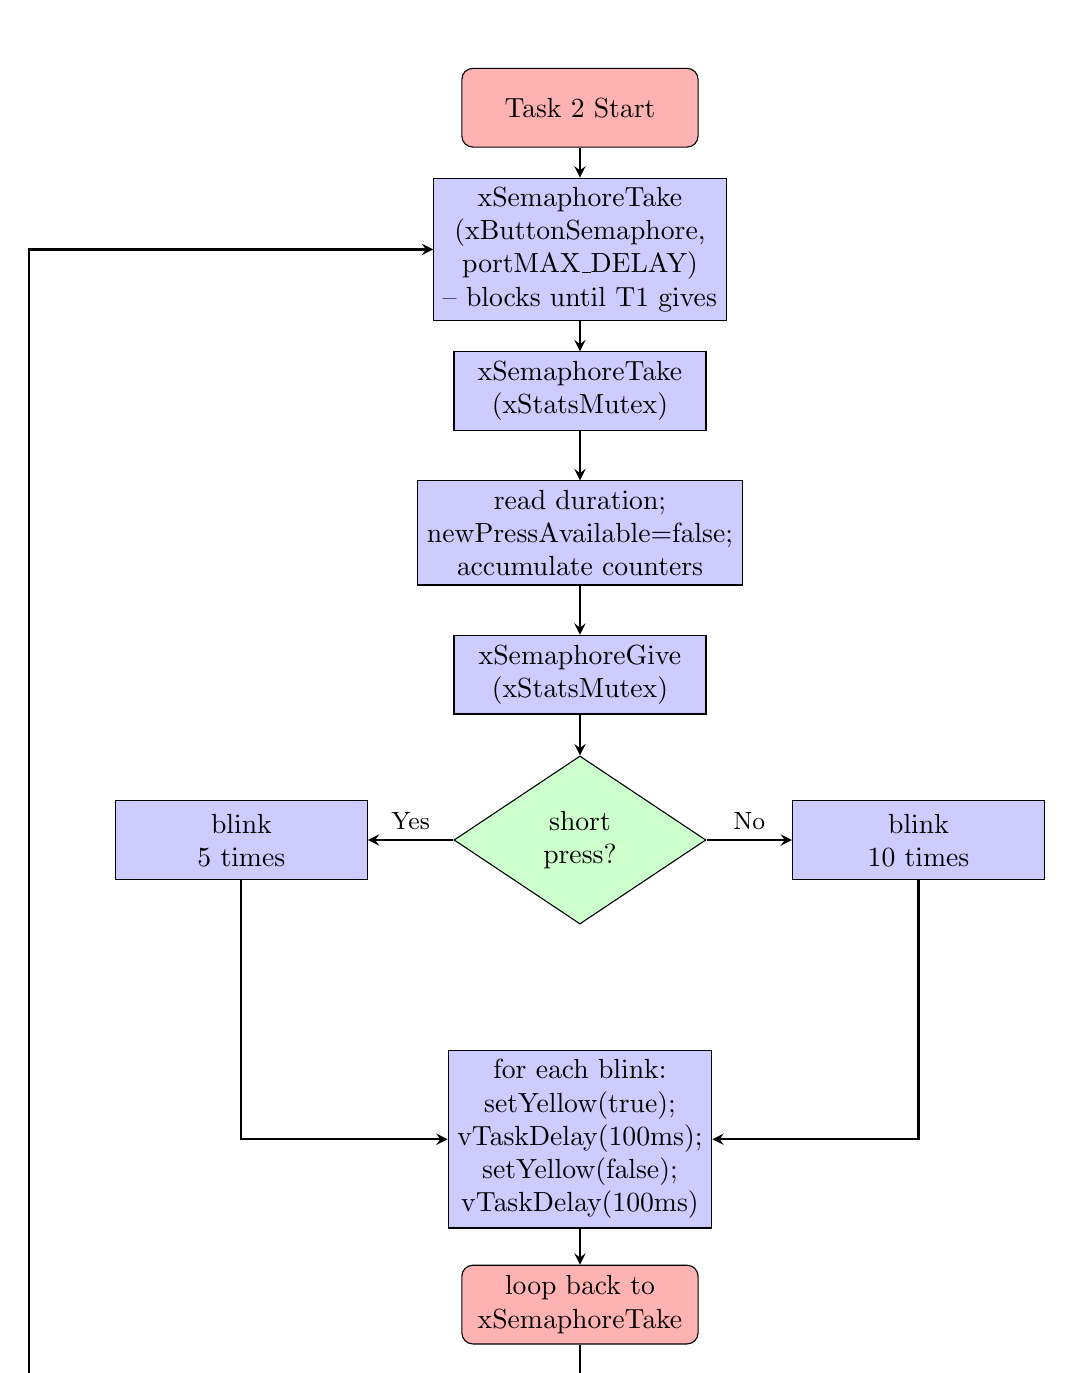
\begin{tikzpicture}[node distance=1.8cm]
    \node (s)   [startstop] {Task 2 Start};
    \node (blk) [process,   below of=s]   {xSemaphoreTake\\(xButtonSemaphore,\\portMAX\_DELAY)\\-- blocks until T1 gives};
    \node (mtx) [process,   below of=blk] {xSemaphoreTake\\(xStatsMutex)};
    \node (acc) [process,   below of=mtx] {read duration;\\newPressAvailable=false;\\accumulate counters};
    \node (rel) [process,   below of=acc] {xSemaphoreGive\\(xStatsMutex)};
    \node (bl)  [decision,  below of=rel,  yshift=-0.3cm] {short\\press?};
    \node (b5)  [process,   left  of=bl,   xshift=-2.5cm] {blink\\5 times};
    \node (b10) [process,   right of=bl,   xshift=2.5cm]  {blink\\10 times};
    \node (lp)  [process,   below of=bl,   yshift=-2.0cm] {for each blink:\\setYellow(true);\\vTaskDelay(100ms);\\setYellow(false);\\vTaskDelay(100ms)};
    \node (rep) [startstop, below of=lp,   yshift=-0.3cm] {loop back to\\xSemaphoreTake};

    \draw [arrow] (s)   -- (blk);
    \draw [arrow] (blk) -- (mtx);
    \draw [arrow] (mtx) -- (acc);
    \draw [arrow] (acc) -- (rel);
    \draw [arrow] (rel) -- (bl);
    \draw [arrow] (bl)  -- node[above]{\small Yes} (b5);
    \draw [arrow] (bl)  -- node[above]{\small No}  (b10);
    \draw [arrow] (b5.south)  |- (lp.west);
    \draw [arrow] (b10.south) |- (lp.east);
    \draw [arrow] (lp)  -- (rep);
    \draw [arrow] (rep.south) -- ++(0,-0.5) -| ++(-7,0) |- (blk.west);
\end{tikzpicture}
\caption{Task 2 flowchart -- event-driven statistics and yellow LED blink}
\label{fig:task2flow}
\end{figure}

\subsubsection{Task 3 Flowchart (FreeRTOS)}

\begin{figure}[h!]
\centering
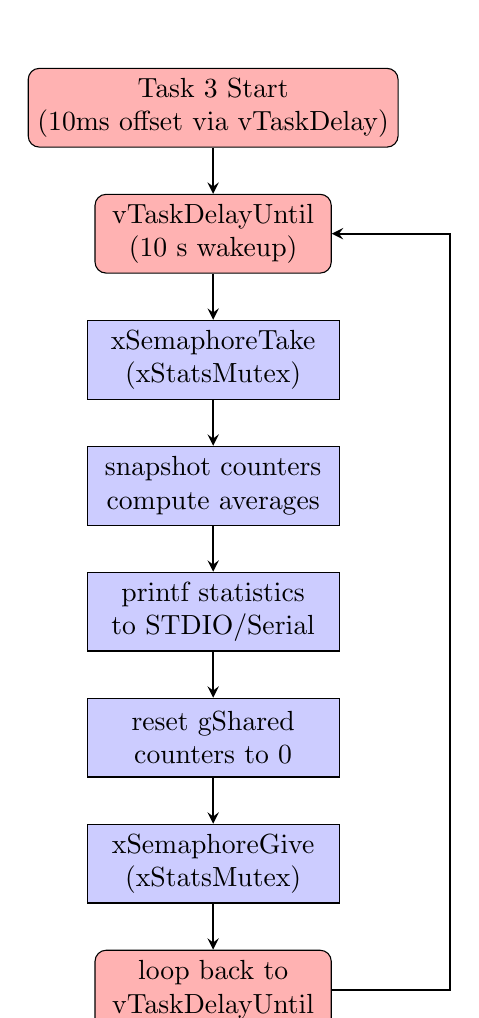
\begin{tikzpicture}[node distance=1.6cm]
    \node (s)   [startstop] {Task 3 Start\\(10ms offset via vTaskDelay)};
    \node (wu)  [startstop, below of=s]   {vTaskDelayUntil\\(10 s wakeup)};
    \node (mtx) [process,   below of=wu]  {xSemaphoreTake\\(xStatsMutex)};
    \node (snap)[process,   below of=mtx] {snapshot counters\\compute averages};
    \node (prt) [process,   below of=snap]{printf statistics\\to STDIO/Serial};
    \node (rst) [process,   below of=prt] {reset gShared\\counters to 0};
    \node (rel) [process,   below of=rst] {xSemaphoreGive\\(xStatsMutex)};
    \node (ret) [startstop, below of=rel] {loop back to\\vTaskDelayUntil};

    \draw [arrow] (s)   -- (wu);
    \draw [arrow] (wu)  -- (mtx);
    \draw [arrow] (mtx) -- (snap);
    \draw [arrow] (snap)-- (prt);
    \draw [arrow] (prt) -- (rst);
    \draw [arrow] (rst) -- (rel);
    \draw [arrow] (rel) -- (ret);
    \draw [arrow] (ret.east) -- ++(1.5,0) |- (wu.east);
\end{tikzpicture}
\caption{Task 3 flowchart -- periodic STDIO statistics report under mutex}
\label{fig:task3flow}
\end{figure}

\subsubsection{FreeRTOS Execution Timeline}

The diagram below shows task state transitions over $\approx$\,60\,ms featuring one short button press at $t=20$\,ms. Task\,1 runs every 20\,ms; Task\,2 wakes only when signalled.

\begin{figure}[htbp]
\centering
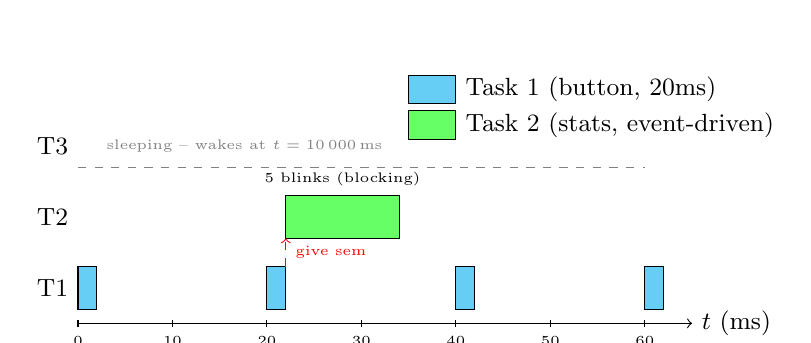
\begin{tikzpicture}[x=0.12cm, y=0.9cm]
  % Time axis
  \draw[->] (0,0) -- (65,0) node[right]{\small $t$ (ms)};
  \foreach \x in {0,10,20,30,40,50,60}
      \draw (\x,0.05) -- (\x,-0.05) node[below]{\tiny \x};

  % Task 1 bars: period=20, offset=0, width~2ms
  \foreach \s in {0,20,40,60}
      \filldraw[fill=cyan!60,draw=black] (\s,0.2) rectangle (\s+2,0.8);
  \node[left] at (0,0.5) {\small T1};

  % Task 2 bar: wakes at ~22ms (after T1 at t=20 gives semaphore), width~12ms (5 blinks x 200ms = 1000ms but compressed)
  \filldraw[fill=green!60,draw=black] (22,1.2) rectangle (34,1.8);
  \node[left] at (0,1.5) {\small T2};
  \node[above,font=\tiny] at (28,1.8) {5 blinks (blocking)};

  % Task 3: sleeping (dashed line)
  \node[left] at (0,2.5) {\small T3};
  \draw[dashed,gray] (0,2.2) -- (60,2.2);
  \node[right,gray,font=\tiny] at (2,2.5) {sleeping -- wakes at $t=10\,000$\,ms};

  % Semaphore event annotation
  \draw[->,dashed,red] (22,0.8) -- node[right,font=\tiny,red]{give sem} (22,1.2);

  % Legend
  \filldraw[fill=cyan!60]  (35,3.1) rectangle (40,3.5); \node[right,font=\small] at (40,3.3){Task 1 (button, 20ms)};
  \filldraw[fill=green!60] (35,2.6) rectangle (40,3.0); \node[right,font=\small] at (40,2.8){Task 2 (stats, event-driven)};
\end{tikzpicture}
\caption{FreeRTOS task execution timeline -- short press at $t=20$\,ms}
\label{fig:timing}
\end{figure}

\subsubsection{Sequence Diagram}

\begin{figure}[htbp]
\centering
\resizebox{\textwidth}{!}{%
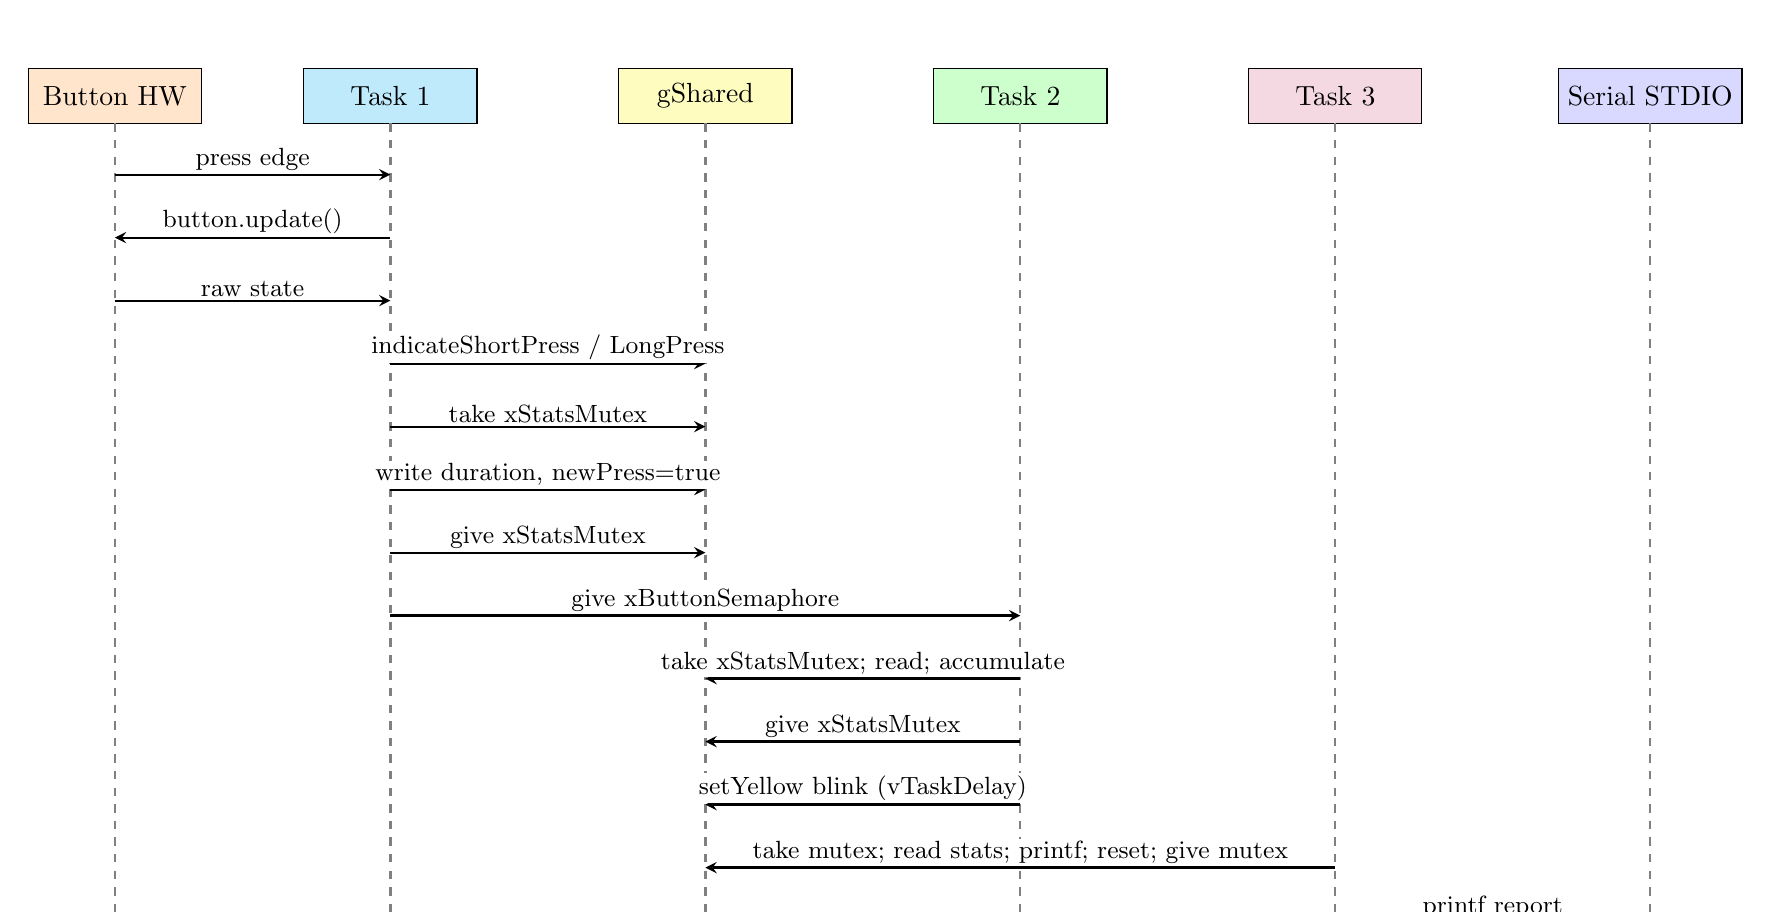
\begin{tikzpicture}[
    lifeline/.style={thick},
    msg/.style={->,>=stealth,thick},
    lbl/.style={font=\small,fill=white,inner sep=1pt}
]
  \node (HW)   at (0,   0) [draw, fill=orange!20, minimum width=2.2cm, minimum height=0.7cm] {Button HW};
  \node (T1)   at (3.5, 0) [draw, fill=cyan!25,   minimum width=2.2cm, minimum height=0.7cm] {Task 1};
  \node (SH)   at (7.5, 0) [draw, fill=yellow!25, minimum width=2.2cm, minimum height=0.7cm] {gShared};
  \node (T2)   at (11.5,0) [draw, fill=green!20,  minimum width=2.2cm, minimum height=0.7cm] {Task 2};
  \node (T3)   at (15.5,0) [draw, fill=purple!15, minimum width=2.2cm, minimum height=0.7cm] {Task 3};
  \node (SER)  at (19.5,0) [draw, fill=blue!15,   minimum width=2.2cm, minimum height=0.7cm] {Serial STDIO};

  \foreach \x in {0,3.5,7.5,11.5,15.5,19.5}
      \draw[lifeline,dashed,gray] (\x,-0.35) -- (\x,-10.5);

  \draw[msg] (0,-1.0)   -- node[lbl,above]{press edge}                      (3.5,-1.0);
  \draw[msg] (3.5,-1.8) -- node[lbl,above]{button.update()}                 (0,-1.8);
  \draw[msg] (0,-2.6)   -- node[lbl,above]{raw state}                       (3.5,-2.6);
  \draw[msg] (3.5,-3.4) -- node[lbl,above]{indicateShortPress / LongPress}  (7.5,-3.4);
  \draw[msg] (3.5,-4.2) -- node[lbl,above]{take xStatsMutex}                (7.5,-4.2);
  \draw[msg] (3.5,-5.0) -- node[lbl,above]{write duration, newPress=true}   (7.5,-5.0);
  \draw[msg] (3.5,-5.8) -- node[lbl,above]{give xStatsMutex}                (7.5,-5.8);
  \draw[msg] (3.5,-6.6) -- node[lbl,above]{give xButtonSemaphore}           (11.5,-6.6);
  \draw[msg] (11.5,-7.4)-- node[lbl,above]{take xStatsMutex; read; accumulate} (7.5,-7.4);
  \draw[msg] (11.5,-8.2)-- node[lbl,above]{give xStatsMutex}                (7.5,-8.2);
  \draw[msg] (11.5,-9.0)-- node[lbl,above]{setYellow blink (vTaskDelay)}    (7.5,-9.0);
  \draw[msg] (15.5,-9.8)-- node[lbl,above]{take mutex; read stats; printf; reset; give mutex} (7.5,-9.8);
  \draw[msg] (15.5,-10.5)-- node[lbl,above]{printf report}                  (19.5,-10.5);
\end{tikzpicture}%
}%
\caption{Sequence diagram -- FreeRTOS inter-task communication on button press}
\label{fig:sequence}
\end{figure}

\subsubsection{Full System State Machine}

\begin{figure}[htbp]
\centering
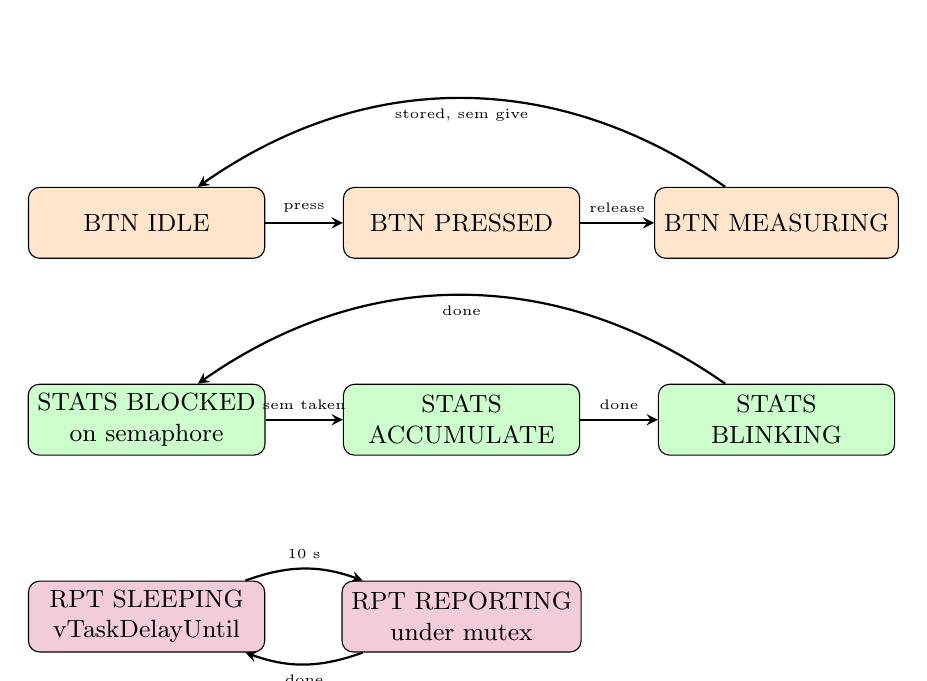
\begin{tikzpicture}[
    state/.style={rectangle, rounded corners, draw, fill=blue!12,
                  minimum width=3.0cm, minimum height=0.9cm, font=\small}
]
  % --- Button driver FSM ---
  \node[state, fill=orange!20] (BW) at (0,    0)  {BTN IDLE};
  \node[state, fill=orange!20] (BP) at (4.0,  0)  {BTN PRESSED};
  \node[state, fill=orange!20] (BM) at (8.0,  0)  {BTN MEASURING};
  \draw[arrow] (BW) -- node[above]{\tiny press}   (BP);
  \draw[arrow] (BP) -- node[above]{\tiny release} (BM);
  \draw[arrow] (BM) to[bend right=35] node[below]{\tiny stored, sem give} (BW);

  % --- Task 2 state ---
  \node[state, fill=green!20]  (STID)  at (0,   -2.5) {STATS BLOCKED\\on semaphore};
  \node[state, fill=green!20]  (STACC) at (4.0, -2.5) {STATS\\ACCUMULATE};
  \node[state, fill=green!20]  (STBL)  at (8.0, -2.5) {STATS\\BLINKING};
  \draw[arrow] (STID)  -- node[above]{\tiny sem taken} (STACC);
  \draw[arrow] (STACC) -- node[above]{\tiny done}      (STBL);
  \draw[arrow] (STBL)  to[bend right=35] node[below]{\tiny done} (STID);

  % --- Task 3 state ---
  \node[state, fill=purple!20] (RSLP) at (0,   -5.0) {RPT SLEEPING\\vTaskDelayUntil};
  \node[state, fill=purple!20] (RRPT) at (4.0, -5.0) {RPT REPORTING\\under mutex};
  \draw[arrow] (RSLP) to[bend left=20]  node[above]{\tiny 10 s} (RRPT);
  \draw[arrow] (RRPT) to[bend left=20]  node[below]{\tiny done} (RSLP);
\end{tikzpicture}
\caption{Full system state machine -- button driver and both consumer tasks}
\label{fig:fsm-full}
\end{figure}

\subsection{Test Scenarios and Validation Criteria}

\begin{longtable}{p{1.0cm} p{2.3cm} p{4.5cm} p{4.5cm} p{1.0cm}}
\toprule
\textbf{ID} & \textbf{Category} & \textbf{Scenario} & \textbf{Expected result} & \textbf{Req.} \\
\midrule
\endfirsthead
T-01 & Button & Press $\approx$\,200\,ms then release & Green LED ON within 20\,ms; stays ON 800\,ms & R-F-01--03 \\
T-02 & Button & Press $\approx$\,1\,000\,ms then release & Red LED ON within 20\,ms; stays ON 800\,ms & R-F-01, R-F-04 \\
T-03 & LED blink & Short press & Yellow blinks exactly 5 times at 100\,ms cadence & R-F-06 \\
T-04 & LED blink & Long press & Yellow blinks exactly 10 times at 100\,ms cadence & R-F-07 \\
T-05 & Statistics & 3 short + 2 long in one 10\,s window & Serial: total=5, short=3, long=2; averages correct & R-F-05, R-F-08 \\
T-06 & Reset & After report & Next 10\,s window starts from counters = 0 & R-F-09 \\
T-07 & Idle & No presses in 10\,s & Report total=0; no division-by-zero & R-F-08 \\
T-08 & Debounce & Rapid noise ($<$\,20\,ms) & No press registered & R-F-01 \\
T-09 & Concurrency & Task 2 blinks while Task 3 reports simultaneously & Counters consistent; no corruption & R-F-10, R-F-11 \\
T-10 & Semaphore & Task 2 wakes only after Task 1 gives semaphore & Task 2 idle (blocked) with no button activity & R-F-10 \\
T-11 & Mutex & Task 3 reads while Task 2 writes & No torn reads; report values match pressed count & R-F-11 \\
T-12 & Latency & Button press to LED on & $<$\,100\,ms & R-NF-01 \\
T-13 & STDIO & printf output format & Lines terminated correctly; no stair-step & R-NF-04 \\
T-14 & Memory & Build size & Flash $<$ 32\,KB, RAM $<$ 2\,KB & R-NF-02 \\
\bottomrule
\caption{Test scenarios and validation criteria}
\label{tab:tests}
\end{longtable}

\subsection{Design Phase Conclusions}
\hspace{0.8cm} The design establishes a clean FreeRTOS-only architecture that maximises idle CPU time through blocking synchronisation primitives. The binary semaphore replaces the bare-metal \texttt{newPressAvailable} polling flag with a zero-overhead blocking wait, and the mutex correctly scopes the shared statistics struct access window to the minimum critical section duration. The \texttt{vTaskDelayUntil} pattern in Tasks\,1 and 3 provides drift-free periodic scheduling regardless of task execution time variation -- an important property for long-running systems.

The STDIO bridge design using \texttt{fdev\_setup\_stream} + \texttt{ultoa} was dictated by the AVR stack constraint: the full \texttt{vfprintf} long-integer formatter would overflow the 400-byte report task stack, causing FreeRTOS state corruption and system-wide failure.

% ---------------------------------------------------------------------------
% SECTION 3 — IMPLEMENTATION
% ---------------------------------------------------------------------------
\section{Hardware and Software Implementation}

\subsection{Electrical Schematic}

\begin{figure}[h!]
\centering
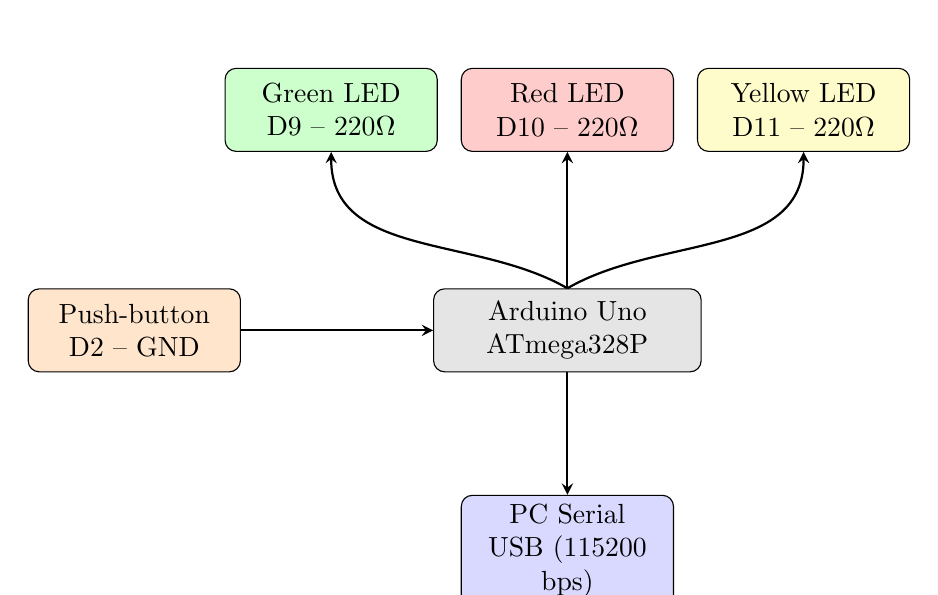
\begin{tikzpicture}
    \node (uno)  at (5.5, 0)    [block, fill=gray!20, text width=9em]
          {Arduino Uno\\ATmega328P};
    \node (btn)  at (0,   0)    [block, fill=orange!20] {Push-button\\D2 -- GND};
    \node (gled) at (2.5, 2.8)  [block, fill=green!20]  {Green LED\\D9 -- 220$\Omega$};
    \node (rled) at (5.5, 2.8)  [block, fill=red!20]    {Red LED\\D10 -- 220$\Omega$};
    \node (yled) at (8.5, 2.8)  [block, fill=yellow!20] {Yellow LED\\D11 -- 220$\Omega$};
    \node (ser)  at (5.5, -2.8) [block, fill=blue!15]   {PC Serial\\USB (115200 bps)};

    \draw [arrow] (btn.east)  -- (uno.west);
    \draw [arrow] (uno.north) to[out=150,in=270] (gled.south);
    \draw [arrow] (uno.north) -- (rled.south);
    \draw [arrow] (uno.north) to[out=30,in=270]  (yled.south);
    \draw [arrow] (uno.south) -- (ser.north);
\end{tikzpicture}
\caption{Functional electrical interconnection sketch}
\label{fig:electrical-func}
\end{figure}

\textbf{Pin assignment:}
\begin{itemize}
    \item D2 -- Push-button (INPUT\_PULLUP; other side to GND)
    \item D9 -- Green LED + 220\,$\Omega$ resistor
    \item D10 -- Red LED + 220\,$\Omega$ resistor
    \item D11 -- Yellow LED + 220\,$\Omega$ resistor
    \item TX/D1 -- Serial UART to USB/PC at 115\,200 baud
\end{itemize}

\begin{figure}[h!]
\centering
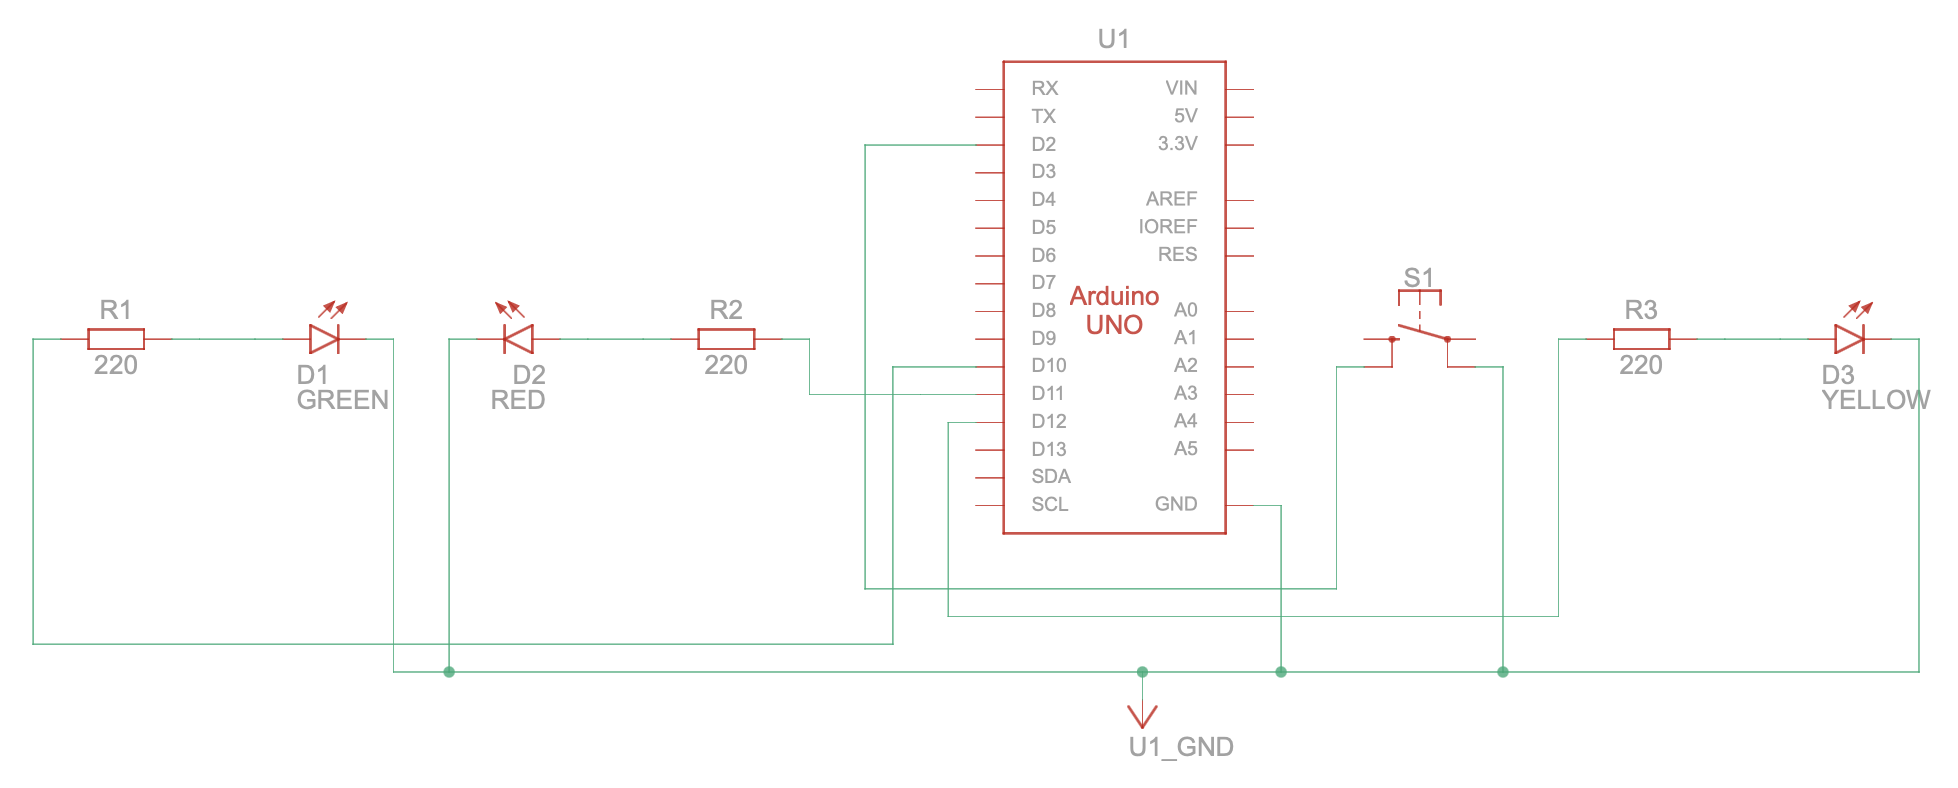
\includegraphics[width=0.85\textwidth]{electrical_circuit.png}
\caption{Electrical circuit diagram -- Wokwi schematic}
\label{fig:electrical-circuit}
\end{figure}

\begin{figure}[htbp]
\centering
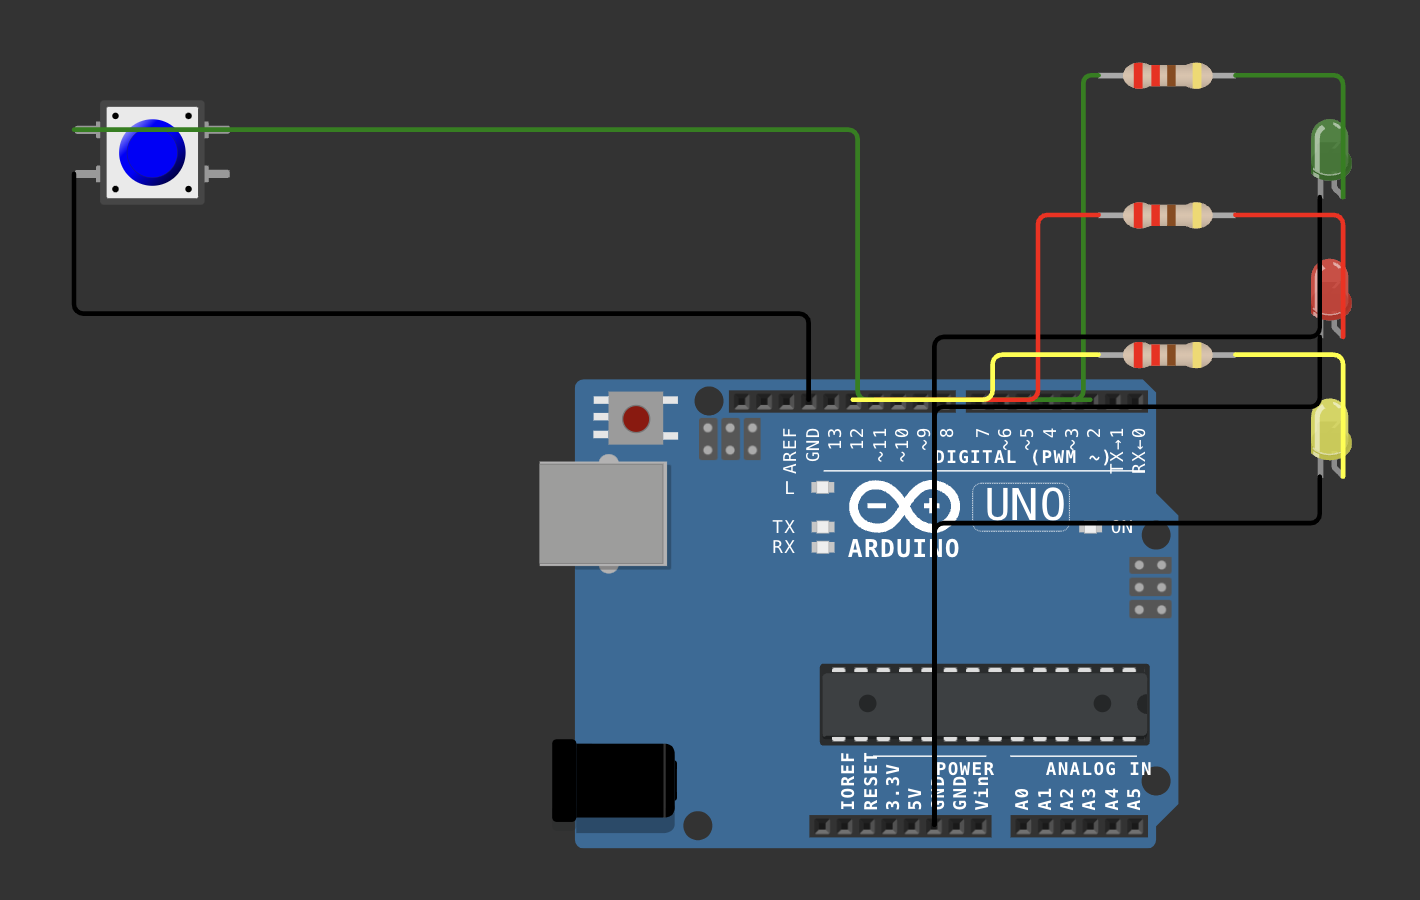
\includegraphics[width=0.85\textwidth]{off.png}
\caption{Wokwi simulation circuit (simulation off)}
\label{fig:wokwi-circuit}
\end{figure}

\subsection{Project Directory Structure}

\begin{verbatim}
lab4/
|-- platformio.ini          <- single env: freertos (feilipu/FreeRTOS@^11.1.0-3)
|-- diagram.json            <- Wokwi circuit definition
|-- wokwi.toml              <- Wokwi firmware pointer (.pio/build/freertos/)
|-- src/
|   |-- main.cpp            <- FreeRTOS setup(): sync primitives + xTaskCreate
|   |-- config/
|   |   `-- AppConfig.h     <- all pins, thresholds, timing, stack sizes
|   |-- shared/
|   |   |-- SharedData.h    <- inter-task state struct (gShared)
|   |   `-- SharedData.cpp
|   |-- peripherals/
|   |   |-- ButtonInput.h/.cpp   <- ECAL debounce FSM driver
|   |   `-- LedController.h/.cpp <- ECAL three-LED driver
|   `-- tasks/
|       |-- TaskButtonMeasure.h/.cpp  <- Task 1 (FreeRTOS)
|       |-- TaskStatistics.h/.cpp     <- Task 2 (FreeRTOS)
|       `-- TaskReport.h/.cpp         <- Task 3 (FreeRTOS)
`-- report/
    `-- main.tex
\end{verbatim}

Lab\,4 has a simpler structure than Lab\,3: there is no \texttt{os/Scheduler} module (FreeRTOS replaces it entirely), no dual entry-point files, and no bare-metal conditional compilation guards.

\subsection{Software Module Descriptions}

\begin{itemize}
    \item \textbf{AppConfig.h}: Central configuration header. Pin assignments, timing constants, blink counts, FreeRTOS stack sizes (words), and task priorities. Changing one constant propagates to all modules. \texttt{StackReport = 200} words accounts for \texttt{printf} call overhead.

    \item \textbf{SharedData}: Plain C struct \texttt{gShared} with \texttt{volatile} fields for inter-task state. Every access in Tasks\,1, 2 and 3 is bracketed by \texttt{xSemaphoreTake(xStatsMutex)} / \texttt{xSemaphoreGive(xStatsMutex)}.

    \item \textbf{ButtonInput}: Four-state debounce FSM. \texttt{update(nowMs)} advances the state machine without blocking. \texttt{wasReleased()} is a one-shot flag cleared at the start of each \texttt{update()} call to prevent double-counting.

    \item \textbf{LedController}: ECAL wrapper exposing \texttt{indicateShortPress()}, \texttt{indicateLongPress()}, \texttt{setYellow(bool)}, \texttt{clearIndicator()}. No timing logic.

    \item \textbf{TaskButtonMeasure}: FreeRTOS task running at 20\,ms via \texttt{vTaskDelayUntil}. Reads \texttt{millis()} for FSM and indicator-LED timeout management. On release: takes mutex, writes \texttt{gShared}, gives mutex, gives \texttt{xButtonSemaphore}.

    \item \textbf{TaskStatistics}: Event-driven FreeRTOS task. Blocks on \texttt{xButtonSemaphore (portMAX\_DELAY)} -- completely idle (zero CPU) until Task\,1 fires. Takes mutex, reads and accumulates \texttt{gShared}, gives mutex. Then blinks yellow using \texttt{vTaskDelay} loop -- blocking is safe here because the task has no periodic deadline.

    \item \textbf{TaskReport}: 10\,s periodic FreeRTOS task. After the initial 10\,ms offset (\texttt{vTaskDelay}), uses \texttt{vTaskDelayUntil} for drift-free wakeup. Takes \texttt{xStatsMutex}, snapshots counters, computes integer averages, prints with \texttt{printf} via the STDIO bridge, resets counters, gives mutex. Uses \texttt{ultoa()} for each \texttt{uint32\_t} value to avoid the AVR long-integer \texttt{vfprintf} stack overflow.

    \item \textbf{main.cpp / STDIO bridge}: \texttt{serial\_putchar} translates \texttt{stdout} writes to \texttt{Serial.write()} with automatic \texttt{\textbackslash{}n} $\rightarrow$ \texttt{\textbackslash{}r\textbackslash{}n} conversion. Registered via \texttt{fdev\_setup\_stream} before \texttt{vTaskStartScheduler()} so all tasks inherit it.
\end{itemize}

\subsection{Critical Code Sections}

The complete source code for the FreeRTOS environment is available on GitHub:

\medskip
\noindent\textbf{Repository:} \url{https://github.com/Ekkusuu/embedded-systems-repo/tree/main/lab4}

\subsection{Implementation Phase Conclusions}
\hspace{0.8cm} The FreeRTOS implementation cleanly separated hardware, shared state, and task logic into independent modules. The event-driven Task\,2 design eliminates all polling, and the mutex ensures that Task\,3's 10-second snapshot always sees a consistent set of counters even if Task\,2 is mid-accumulation.

Two key lessons emerged during implementation:
\begin{enumerate}
    \item The AVR \texttt{printf(\%lu)} formatter silently overflows a small FreeRTOS task stack, causing corruption that kills all tasks after a few report cycles. The safe solution is \texttt{ultoa()} + \texttt{printf(\%s)} which requires only the string-format \texttt{vfprintf} path.
    \item \texttt{vTaskDelayUntil} must be called \emph{after} obtaining \texttt{xLastWakeTime = xTaskGetTickCount()} (not before), otherwise the first wakeup interval is undefined.
\end{enumerate}

% ---------------------------------------------------------------------------
% SECTION 4 — TESTING AND VALIDATION
% ---------------------------------------------------------------------------
\section{Testing and Validation}

\subsection{Build Results}

\begin{table}[h!]
\centering
\begin{tabular}{lrrrr}
\toprule
\textbf{Environment} & \textbf{Flash used} & \textbf{Flash \%} & \textbf{RAM used} & \textbf{RAM \%} \\
\midrule
\texttt{freertos} & 13\,956 B & 43.3\% & 791 B & 38.6\% \\
\bottomrule
\end{tabular}
\caption{PlatformIO build resource usage (Lab 4)}
\label{tab:build}
\end{table}

The build completes with \texttt{[SUCCESS]}, zero errors, zero warnings. Flash and RAM usage remain well within the ATmega328P limits (R-NF-02 satisfied). The increased RAM usage relative to Lab\,3's FreeRTOS build (424\,B) reflects the larger \texttt{StackReport} value (200 versus 90 words) required for safe \texttt{printf} execution.

\subsection{Test Execution Report}

\begin{longtable}{p{0.8cm} p{3.5cm} p{6.5cm} p{1.5cm}}
\toprule
\textbf{ID} & \textbf{Scenario} & \textbf{Observed result} & \textbf{Result} \\
\midrule
\endhead
T-01 & Short press $\approx$\,200\,ms & Green LED illuminates within one 20\,ms task cycle & PASS \\
T-02 & Long press $\approx$\,1\,000\,ms & Red LED illuminates; extinguishes after 800\,ms & PASS \\
T-03 & Yellow blink short & 5 blinks counted at 100\,ms ON/OFF cadence & PASS \\
T-04 & Yellow blink long & 10 blinks counted at 100\,ms ON/OFF cadence & PASS \\
T-05 & 3 short + 2 long & Serial: total=5, short=3, long=2; averages correct & PASS \\
T-06 & Counter reset & Second window starts from counters = 0 & PASS \\
T-07 & Idle 10\,s & Report total=0; no crash on zero-division guard & PASS \\
T-08 & Bounce noise & No spurious count; debounce filters transient & PASS \\
T-09 & Concurrency & Yellow blink and STDIO report co-exist; counters consistent & PASS \\
T-10 & Semaphore block & Task 2 confirmed idle (blocked) with no button activity & PASS \\
T-11 & Mutex integrity & Report values match pressed count; no torn reads & PASS \\
T-12 & Latency & LED responds within 20\,ms of stable press & PASS \\
T-13 & STDIO format & Lines left-aligned; correct \texttt{\textbackslash{}r\textbackslash{}n} line endings & PASS \\
T-14 & Memory & Flash 43.3\%, RAM 38.6\% (both $<$ 100\%) & PASS \\
\bottomrule
\caption{Test execution results -- FreeRTOS environment}
\label{tab:testresults}
\end{longtable}

All 14 tests passed. Of particular note: T-09 and T-11 confirm that the mutex correctly serialises concurrent access to \texttt{gShared} between Tasks\,2 and 3, and T-10 confirms that Task\,2 consumes no CPU while waiting for a button event -- a core FreeRTOS efficiency property.

\subsection{Hardware Assembly}

The circuit was assembled on a breadboard using an Arduino Uno, a tactile push-button, three discrete LEDs (green, red, yellow) with 220\,$\Omega$ resistors. Pin assignments match the Wokwi simulation schematic identically.

\begin{figure}[htbp]
\centering
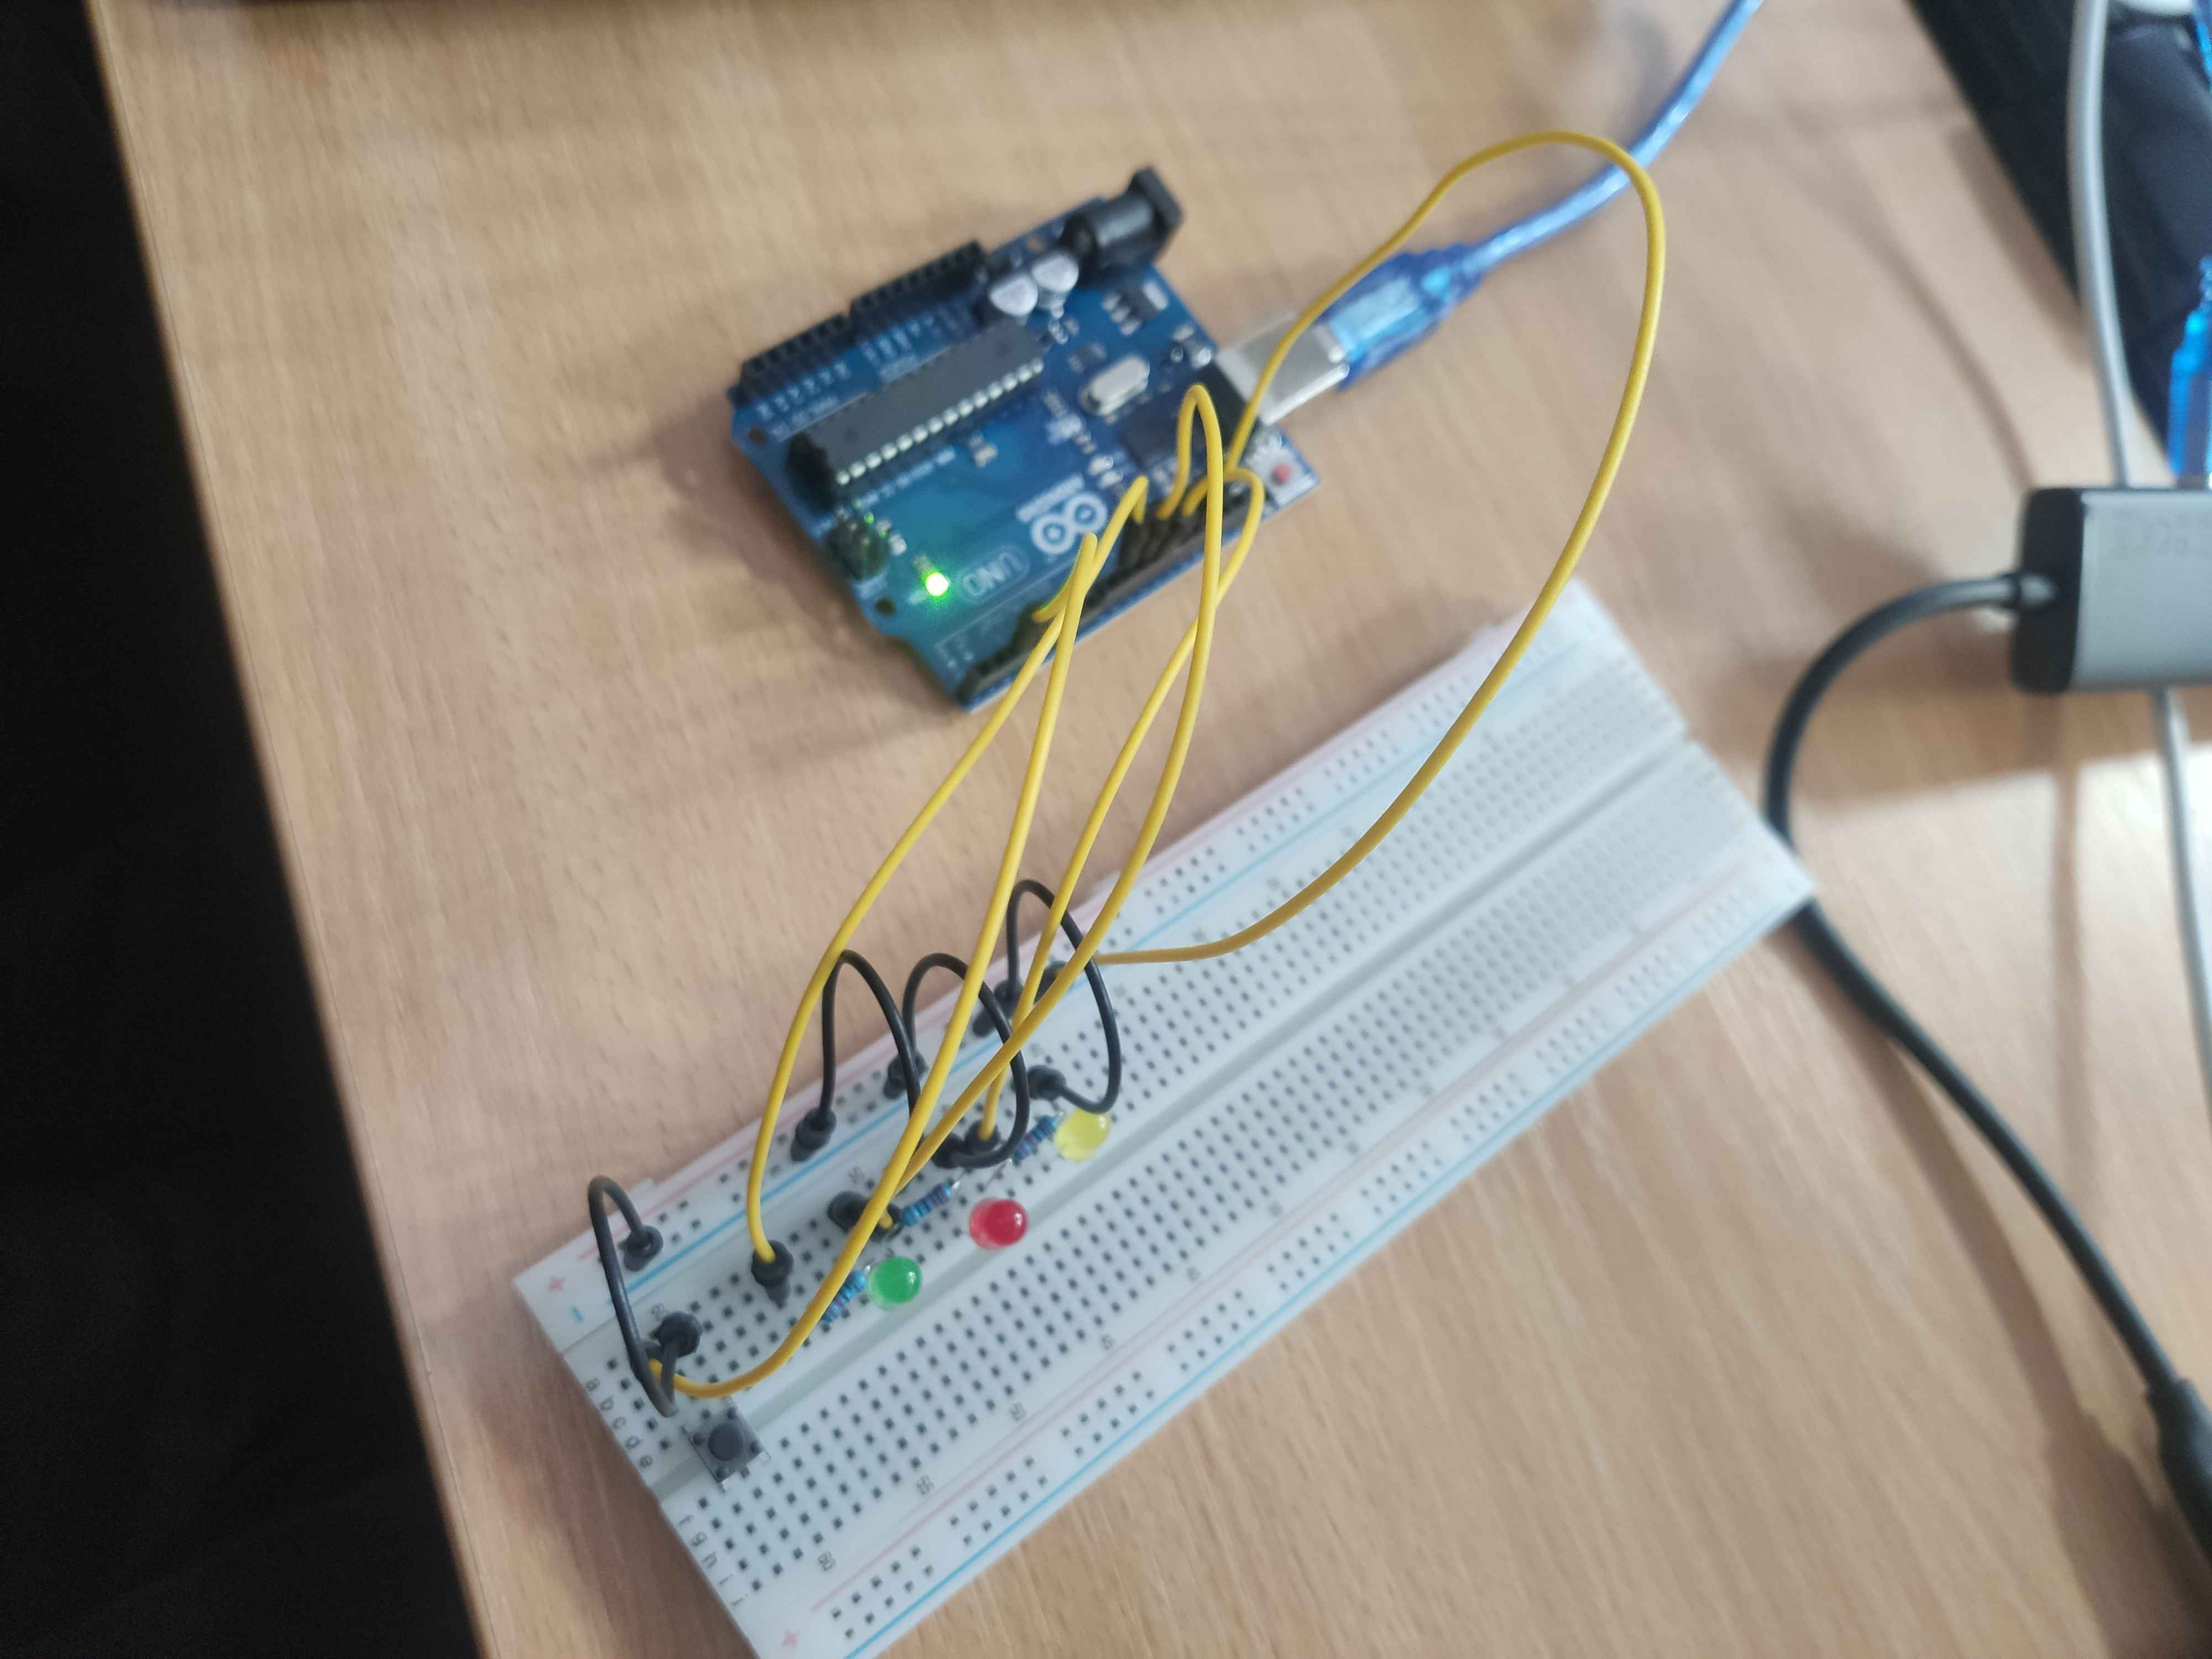
\includegraphics[width=0.85\textwidth]{irl_setup.jpg}
\caption{Physical hardware assembly -- Arduino Uno with debounced button and three-LED indicator circuit}
\label{fig:hw-photo}
\end{figure}

\subsection{Simulation Screenshots}

\begin{figure}[htbp]
\centering
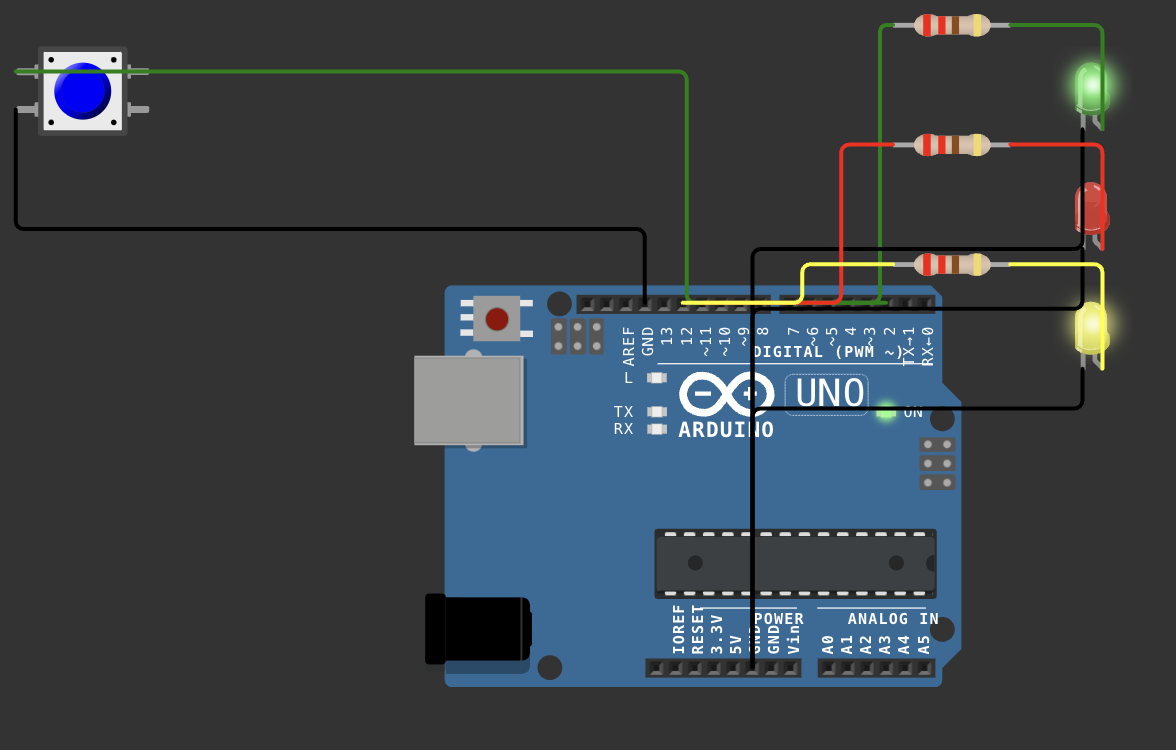
\includegraphics[width=0.85\textwidth]{short_press.png}
\caption{Wokwi simulation: short press -- Green LED illuminated}
\label{fig:wokwi-short}
\end{figure}

\begin{figure}[htbp]
\centering
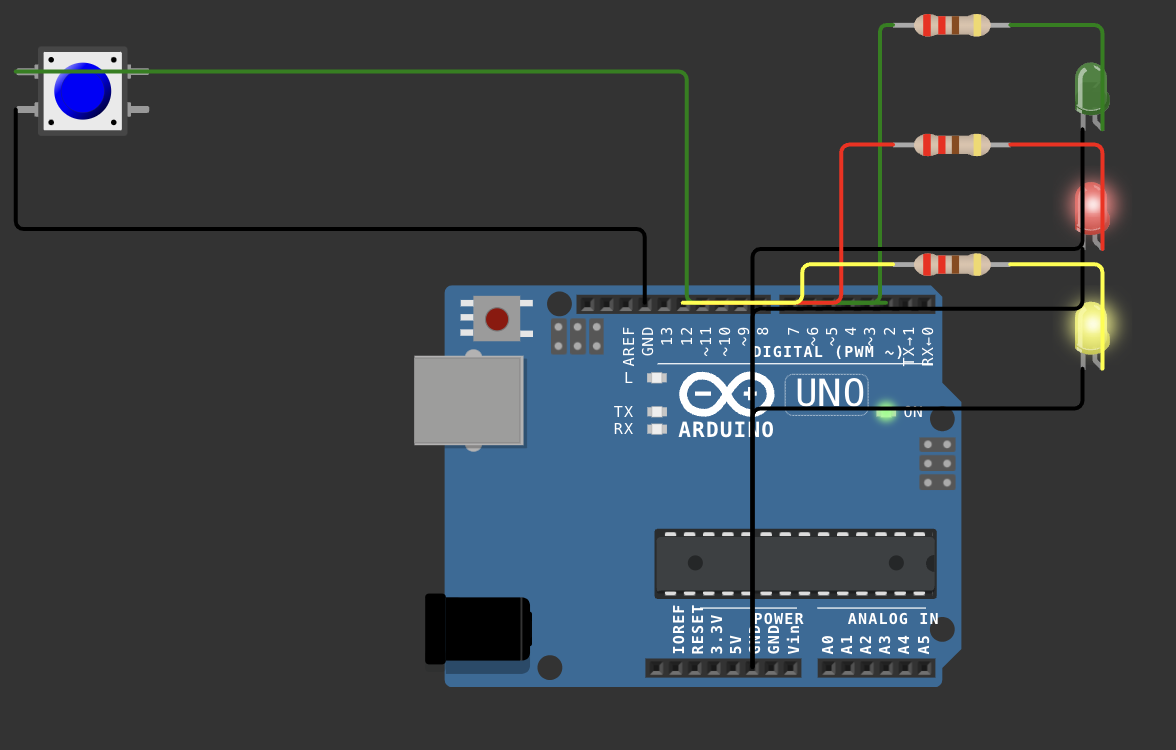
\includegraphics[width=0.85\textwidth]{long_press.png}
\caption{Wokwi simulation: long press -- Red LED illuminated}
\label{fig:wokwi-long}
\end{figure}

\begin{figure}[htbp]
\centering

\includegraphics[width=0.85\textwidth]{terminal.png}
\caption{Wokwi serial monitor: periodic statistics report output via printf STDIO}
\label{fig:wokwi-serial}
\end{figure}

\subsection{Representative Serial Output}

The following output was captured from the FreeRTOS build after performing two short presses ($\approx$\,200, 350\,ms) and one long press ($\approx$\,800\,ms):

\begin{verbatim}
Lab 4 - FreeRTOS Preemptive Scheduler
Wiring: BTN=D2  GREEN=D9  RED=D10  YELLOW=D11
Press the button; report prints every 10 s.

========================================
  PERIODIC STATISTICS REPORT (10 s)
========================================
  Total presses     : 3
  Short presses     : 2
  Long  presses     : 1
  Avg short dur [ms]: 275
  Avg long  dur [ms]: 800
  (Counters reset)
========================================
\end{verbatim}

\subsection{Performance Analysis}

\begin{itemize}
    \item \textbf{Button-to-LED latency}: Task\,1 wakes every 20\,ms via \texttt{vTaskDelayUntil}. Maximum latency from button stabilisation to LED change is one period: 20\,ms -- well within R-NF-01 (100\,ms).
    \item \textbf{CPU efficiency}: Task\,2 blocks on \texttt{xButtonSemaphore (portMAX\_DELAY)} and Task\,3 sleeps for 10\,s. Only Task\,1 is periodically active at a 20\,ms rate. During the 20\,ms window, Task\,1 executes in under 10\,$\mu$s -- a CPU load of $<$\,0.05\% per task.
    \item \textbf{Mutex hold time}: The critical sections in Tasks\,1, 2 and 3 are a handful of integer assignments or reads -- typically $<$\,5\,$\mu$s. Priority inversion risk is negligible given the lock durations.
    \item \textbf{Stack headroom}: \texttt{StackReport = 200} words (400\,bytes). The \texttt{printf(\%s)} path requires $\approx$\,150\,bytes. Actual peak usage is estimated at $\approx$\,250\,bytes, leaving 150\,bytes margin -- sufficient for a 16\,MHz AVR with no recursion.
    \item \textbf{FreeRTOS heap}: \texttt{configTOTAL\_HEAP\_SIZE = 950} bytes. Three task stacks (60+60+200 words = 640 bytes) plus FreeRTOS TCBs, semaphore, and mutex blocks consume $\approx$\,800\,bytes -- leaving $\approx$\,150\,bytes free.
\end{itemize}

\subsection{Testing Phase Conclusions}
\hspace{0.8cm} All 14 test scenarios passed, validating every functional and non-functional requirement. The FreeRTOS preemptive architecture demonstrated correct event-driven behaviour: Task\,2 was confirmed to block until woken by the semaphore, and the mutex was verified to prevent data corruption during concurrent Task\,2/Task\,3 access to the statistics struct.

The most notable challenge encountered was the AVR stack overflow triggered by \texttt{printf(\%lu)} -- a subtle AVR-specific issue that does not manifest on 32-bit platforms. The fix (\texttt{ultoa} + \texttt{\%s}) is a lesson applicable to all resource-constrained embedded C/C++ codebases.

% ---------------------------------------------------------------------------
% GENERAL CONCLUSIONS
% ---------------------------------------------------------------------------
\section*{General Conclusions}
\hspace{0.8cm} Laboratory Work \#4 achieved all stated objectives. A complete FreeRTOS preemptive button monitoring application was designed, implemented, and validated on Arduino Uno with three tasks, binary semaphore event signalling, mutex-protected shared state, and printf-based STDIO output.

Key outcomes:
\begin{enumerate}
    \item \textbf{FreeRTOS preemptive scheduling mastery}: Three tasks with different scheduling modes (periodic via \texttt{vTaskDelayUntil}, event-driven via blocking semaphore) co-exist without interference under the FreeRTOS kernel.
    \item \textbf{Binary semaphore event model}: Task\,2 blocks indefinitely with zero CPU consumption until Task\,1 gives the semaphore -- demonstrating the core efficiency advantage of event-driven RTOS programming over bare-metal polling.
    \item \textbf{Mutex-protected shared memory}: The \texttt{xStatsMutex} correctly scopes all \texttt{gShared} accesses, preventing data races between three concurrently executing tasks without introducing significant critical section overhead.
    \item \textbf{vTaskDelayUntil drift correction}: Tasks\,1 and 3 achieve drift-free periodic scheduling regardless of their execution time variability -- a property not achievable with simple \texttt{vTaskDelay}.
    \item \textbf{STDIO via printf}: The \texttt{fdev\_setup\_stream} bridge provides clean separation between formatting logic and hardware output, allowing the report task to use standard C idioms on a bare-metal UART.
    \item \textbf{AVR stack safety}: The \texttt{ultoa + \%s} pattern avoids the 300-byte AVR \texttt{vfprintf} long-integer formatter stack frame, a critical lesson for embedded \texttt{printf} usage.
\end{enumerate}

\textbf{Possible improvements:}
\begin{itemize}
    \item Replace the semaphore + \texttt{gShared.lastPressDurationMs} pattern with a FreeRTOS queue to buffer rapid consecutive presses without data loss.
    \item Add a FreeRTOS software timer for the 800\,ms LED indicator timeout in Task\,1, removing the \texttt{millis()} comparison.
    \item Evaluate \texttt{configUSE\_IDLE\_HOOK = 1} + \texttt{sleep\_cpu()} in the idle hook for power reduction between task wakeups.
\end{itemize}

% ---------------------------------------------------------------------------
% AI TOOL USAGE
% ---------------------------------------------------------------------------
\section*{Note on AI Tool Usage}
\hspace{0.8cm} AI-assisted tools were used to support coding productivity and report drafting:
\begin{itemize}
    \item \textbf{GitHub Copilot} -- code suggestions, FreeRTOS boilerplate, STDIO bridge setup.
    \item \textbf{LLM assistance} -- technical writing structure, language polishing.
\end{itemize}
All generated content was manually reviewed, adapted, compiled, and validated against Wokwi simulation behaviour.

% ---------------------------------------------------------------------------
% BIBLIOGRAPHY
% ---------------------------------------------------------------------------
\section*{Bibliography}
\begin{enumerate}
    \item FreeRTOS Official Documentation -- Mastering the FreeRTOS Real-Time Kernel.\\
    \url{https://www.freertos.org/Documentation/RTOS_book.html}

    \item feilipu/FreeRTOS -- AVR Arduino FreeRTOS port.\\
    \url{https://github.com/feilipu/Arduino_FreeRTOS_Library}

    \item Arduino Official Reference -- GPIO, Serial, \texttt{millis()}.\\
    \url{https://www.arduino.cc/reference/en/}

    \item PlatformIO Documentation -- multi-environment projects and source filters.\\
    \url{https://docs.platformio.org/en/latest/}

    \item AVR-libc Documentation -- \texttt{fdev\_setup\_stream}, \texttt{ultoa}, \texttt{printf}.\\
    \url{https://www.nongnu.org/avr-libc/user-manual/}

    \item Wokwi Simulator Documentation.\\
    \url{https://docs.wokwi.com/}

    \item Lab 4 Theory Notes -- Sisteme de operare pentru sisteme incorporate (Lucrarea 3/4).\\
    Technical University of Moldova, 2026.
\end{enumerate}

% ---------------------------------------------------------------------------
% ANNEX
% ---------------------------------------------------------------------------
\pagebreak
\section*{Annex -- Source Code}

The full source code for the FreeRTOS environment is hosted on GitHub:

\bigskip
\noindent\textbf{Repository URL:}\\
\url{https://github.com/Ekkusuu/embedded-systems-repo/tree/main/lab4}

\bigskip
\noindent This repository contains all source files under \texttt{lab4/src/}, the PlatformIO configuration (\texttt{platformio.ini}), and the Wokwi simulation files (\texttt{diagram.json}, \texttt{wokwi.toml}).

\end{document}
